\documentclass[a4paper,11pt]{book}

\usepackage{graphicx}
\usepackage{caption}
\usepackage{subfigure}
\usepackage{fullpage}
%\usepackage{MinionPro}
\usepackage[scaled=.95]{inconsolata}
\usepackage[Sonny]{fncychap}
\usepackage{fancyhdr}
\usepackage{titlesec}
\usepackage{titling}
\usepackage{xcolor}
\usepackage{listings}
\usepackage{colortbl}
\usepackage{multicol}
\usepackage{multirow}
\usepackage{hhline}
\usepackage{ifpdf}
\ifpdf
\usepackage[protrusion=true,expansion=true]{microtype}
\usepackage{hyperref}
\else
\usepackage{url}
\fi

\renewcommand{\sfdefault}{Myriad-LF}
\renewcommand{\maketitlehooka}{\sf}
\renewcommand{\captionfont}{\small\it}
\renewcommand{\captionlabelfont}{\sf}
\titleformat*{\section}{\sf\Large}
\titleformat*{\subsection}{\sf\large}

\ChNameVar{\Large\sf}
\ChNumVar{\fontsize{60}{1}\selectfont}
\ChTitleVar{\Huge\sf}
\ChRuleWidth{0pt}
\ChNameAsIs

\arrayrulecolor{tableborder}
\renewcommand{\arraystretch}{1.5}
\setlength{\arrayrulewidth}{0.5pt}

\pagestyle{fancy}

\definecolor{lightgray}{RGB}{240,240,240}
\definecolor{darkgray}{RGB}{100,100,100}

\definecolor{tableborder}{RGB}{0,0,0}
\definecolor{tableheader}{RGB}{192,192,193}
\definecolor{tablerow}{RGB}{238,238,238}
\definecolor{tablegray}{RGB}{228,228,230}
\definecolor{tableorange}{RGB}{255,204,50}

\definecolor{hyperrefcite}{RGB}{0,51,153}
\definecolor{hyperrefurl}{RGB}{153,51,51}

\definecolor{codelinenumber}{RGB}{43,145,175}
\definecolor{codekeyword}{RGB}{0,0,255}
\definecolor{codecomment}{RGB}{0,128,0}
\definecolor{codestring}{RGB}{163,21,21}

\lstset{
    basicstyle=\ttfamily\small,
    commentstyle=\color{codecomment},
    stringstyle=\color{codestring},
    keywordstyle=\color{codekeyword},
    xleftmargin=5px,
    xrightmargin=5px,
    framexleftmargin=5px,
    framexrightmargin=5px,
    frame=single,
    backgroundcolor=\color{lightgray},
    rulecolor=\color{tableborder},
    lineskip=-1px,
    showstringspaces=false,
    fontadjust
}

\ifpdf
\hypersetup{
    bookmarks=true,
    unicode=false,
    pdftoolbar=true,
    pdfmenubar=true,
    pdffitwindow=false,
    pdfstartview={FitV},
    pdfpagelayout={TwoPageRight},
    pdftitle={Network Laboratory},
    pdfauthor={Ruizhi Liao, Alex Bikfalvi, Jaume Barcelo, Albert Rabassa},
    pdfsubject={Lab practice},
    pdfcreator={LaTeX2e},
    pdfproducer={Universitat Pompeu Fabra},
    pdfkeywords={traffic} {analysis} {LAN} {WLAN} {VLAN} {STP},
    pdfnewwindow=true,
    colorlinks=true,
    linkcolor=black,
    citecolor=hyperrefcite,
    filecolor=black,
    urlcolor=hyperrefurl
}
\fi

\begin{document}

\frontmatter
\pagestyle{empty}

\title{\Huge Network Laboratory}
\author{Ruizhi Liao, Alex Bikfalvi, Jaume Barcelo, Albert Rabassa}
\date{Spring 2013}
\maketitle

\tableofcontents

\mainmatter

\chapter{About the Course}

\section{Course Data}

Code: 21728

Course name: "Laboratori de Xarxes i Serveis"

Teachers: Ruizhi Liao, Alex Bikfalvi and Jaume Barcelo

Credits: 4

Year: 2nd year

Trimester: Spring

\section{Introduction}

The goal of this course is to acquire hands-on experience with networking equipment such as \emph{access points}, \emph{switches}, \emph{routers} and \emph{firewalls}. The students should be familiar with the high-level functionality of each of these devices. The actual configuration of the equipment and the construction of prototype networks will provide further insights into the operation of these network devices. After the course, the student will be ready to plan and configure a small network.

\section{Syllabus}
\begin{itemize}
  \item Lectures
  \begin{enumerate}
    \item Introduction, Traffic analysis and IEEE 802.11 WLANs
    \item Virtual Local Area Networks and Spanning Tree Protocol
    \item Routers
    \item Firewalls
    \item Test and Final Project
  \end{enumerate}
\item Lab Assignments
  \begin{enumerate}
    \item Traffic analysis
    \item IEEE 802.11 Wireless Local Area Networks (WLANs)
    \item Virtual local area networks (VLANs)
    \item Spanning Tree Protocol (STP)
    \item Routing
    \item Firewalls
  \end{enumerate}
\end{itemize}

\section{Bibliography}

\begin{itemize}
\item J. Kurose, K. Ross, ``Computer Networking''
\item ``Cisco Networking Academy Program: CCNA 1 and 2 companion guide''
\item ``Cisco Networking Academy Program: CCNA 3 and 4 companion guide''
\end{itemize}

\section{Evaluation Criteria}

The final grade is distributed as follows.

\begin{center}
\sffamily\small
\begin{tabular}{l>{\columncolor{tablegray}}l}
\multicolumn{1}{>{\columncolor{tableheader}}c}{Evaluation Method} & \multicolumn{1}{>{\columncolor{tableorange}}c}{Weight}\\
Lab assignments & 70\,\% \\
\hline
Continuous assessment quiz & 10\,\% \\
\hline
Final exam & 20\,\% \\
\hline
\end{tabular}
\end{center}

The students need to obtain a passing mark (half of the available points) in all the different evaluation aspects.

\section{Group Work}

The assignments are done in groups of three students. A single report is delivered for each group. It is important that all the members of the group participate in the experiments and the preparation of the report. The teachers may ask individual questions to the students in the labs, and both the quiz and the final exam are performed individually.

\section{Lab Report}

For each lab assignment, it is necessary to prepare a lab report answering all the questions. The students are also expected to include additional information, explanation and comments besides those explicitly asked in the assignment.

\section{The Lab}
The networking lab has PCs, wireless access points, switches, routers, firewalls and a patch panel to make the connections.
The user for the computers is \texttt{\color{blue}administrador}.
The password for the computers is \texttt{\color{blue}pompeulab}.
The root password for Linux is \texttt{\color{blue}pompeulab}.

\section{Survival guide}

\subsection{Questions and Doubts}

We like to receive questions and comments. Normally, the best moment to express a doubt is during the class, as it is likely that many people in the class share the same doubt. If you feel that you have a question that needs to be discussed privately, we can discuss it right after the class.

\subsection{Continuous Feedback}

At the end of lectures, we will ask you to provide some feedback on the course. In particular, we always want to know:
\begin{itemize}
\item What is the most interesting thing we have seen in class.
\item What is the most confusing thing in the class.
\item Any other comment you may want to add.

\end{itemize}

\subsection{How to Make Your Teachers Happy}

Avoid speaking while we are talking.

\chapter{Traffic Analysis}

\section{Introduction}

The goal of this lab assignment is to learn about monitoring and traffic analysis tools. We shall use the \emph{Wireshark} and \emph{tcpdump} software tools to study different layers of the TCP/IP architecture.

\section{Home Preparation}

Review the TCP/IP model and explain the function of each layer. Provide examples of the protocols at each layer of the protocol stack.

\begin{center}
\sffamily\small
\begin{tabular}{>{\columncolor{tablegray}}p{15cm}}
\multicolumn{1}{>{\columncolor{tableorange}}l}{Questions and Tasks}\\
What is the purpose of ARP? \emph{Tip: Use the RFC826 standard to answer this question \cite{rfc826}.}\\
\hline
Draw a sketch of the different messages being exchanged and the different steps involved.\\
\hline
Is it possible to run this protocol between computers that are in different local area networks (LANs)?\\
\hline
What is the ICMP protocol?\\
\hline
How does the \emph{ping} command work?\\
\hline
What does the \emph{ping} command measure?\\
\hline
Explain and draw an SSL connection indicating how the protocol works and which messages are being exchanged.\\
\hline
\end{tabular}
\end{center}

\section{Disable Your Local Firewall}

On a Linux machine, your local firewall can interfere with the assignment. Disable it using the following command with root permissions.

\begin{lstlisting}
service iptables stop
\end{lstlisting}

\section{Wireshark Network Analyzer}

Start your computer in Linux. Start the \emph{Wireshark} software program and choose the correct network interface from the \textbf{\sf Capture} \textgreater \textbf{\sf Interfaces} dialog. Use it to start the packet capture. It is also possible to configure the length of the capture and other details.

\begin{center}
\sffamily\small
\begin{tabular}{>{\columncolor{tablegray}}p{15cm}}

\multicolumn{1}{>{\columncolor{tableorange}}l}{Questions}\\
What interface does Wireshark detect? What is your IP address? What is the corresponding MAC address?\\
\hline
\end{tabular}
\end{center}

Configure the \textbf{\sf Capture} \textgreater \textbf{\sf Interfaces} options to perform a five minutes capture. Observe the results and answer the following questions.

\begin{center}
\sffamily\small
\begin{tabular}{>{\columncolor{tablegray}}p{15cm}}

\multicolumn{1}{>{\columncolor{tableorange}}l}{Questions}\\
What is the total number of captured packets? Are there lost packets? If yes, why?\\
\hline
\end{tabular}
\end{center}

Select a (any) packet. Observe the details and answer the following questions.

\begin{center}
\sffamily\small
\begin{tabular}{>{\columncolor{tablegray}}p{15cm}}

\multicolumn{1}{>{\columncolor{tableorange}}l}{Questions}\\
What is the source and destination IP address?\\
\hline
What are the source and destination MAC addresses?\\
\hline
What is the number of bytes in the packet?\\
\hline
What protocols can you see in the packet?\\
\hline
Did you capture an HTTP packet? If yes, what is the length of the HTTP message (the payload of the TCP segment or segments)?\\
\hline
What are the source and destination port?\\
\hline
\end{tabular}
\end{center}

In the dialog \textbf{\sf Analyze} \textgreater \textbf{\sf Enable Protocols...} you can configure the protocols that Wireshark captures and displays. Looking at the default protocols, find at least one protocol of each of the four upper layers of the TCP/IP stack (application, transport, internet and link). Include a brief description of the protocols you found.

Select the menu \textbf{\sf Statistics} \textgreater \textbf{\sf Protocol Hierarchy} and observe the percentage of the following protocols: Ethernet, Internet Protocol, TCP, UDP, Logical Link Control, ARP, STP, IPv6, HTTP.

Repeat the previous capture using IPv6, by performing ping to the local-link IPv6 address of a neighbor or attempting an IPv6 ping to an existing destination. You may use one of the following commands:

\begin{lstlisting}
ping6 -I <interface> <address>
\end{lstlisting}
or:
\begin{lstlisting}
ping6 ipv6.google.com
\end{lstlisting}

\begin{center}
\sffamily\small
\begin{tabular}{>{\columncolor{tablegray}}p{15cm}}

\multicolumn{1}{>{\columncolor{tableorange}}l}{Questions}\\
What are the differences between IPv4 and IPv6?\\
\hline
\end{tabular}
\end{center}

\section{The Address Resolution Protocol (ARP)}

The Address Resolution Protocol (ARP) resolves the association between an IP address and a MAC address. It is used in IP over Ethernet networks. Begin a new traffic capture and analyze the ARP packets. You can filter the ARP packets by writing \texttt{\color{blue}ARP} in the \textbf{\sf Filter Toolbar}.

If you do not capture any ARP packets, clear your ARP cache and then ping or browse to any preferred destination. You can use the following command to delete all ARP entries. On a Windows computer use.

\begin{lstlisting}
arp -d *
\end{lstlisting}
On a Linux computer use.

\begin{lstlisting}
sudo ip neighbour flush all
\end{lstlisting}

\begin{center}
\sffamily\small
\begin{tabular}{>{\columncolor{tablegray}}p{15cm}}

\multicolumn{1}{>{\columncolor{tableorange}}l}{Questions}\\
What are the source and destination MAC addresses of the Ethernet frame that contains the ARP request message?\\
\hline
What are the source and destination IP addresses in the ARP request and response frames?\\
\hline
What are the source and destination MAC addresses in the ARP request and response frames?\\
\hline
What is the time elapsing between an ARP request and reply messages?\\
\hline
\end{tabular}
\end{center}

Use the information available in \emph{Wireshark} to indicate the length of the ARP frames and draw the format of the messages.

\begin{center}
\sffamily\small
\begin{tabular}{>{\columncolor{tablegray}}p{15cm}}

\multicolumn{1}{>{\columncolor{tableorange}}l}{Question}\\
To which layer does ARP belong?\\
\hline
\end{tabular}
\end{center}

\section{HTTP and Secure HTTP}

Begin a new 5 minutes capture and during this time visit a few web sites, such as \url{http://www.upf.edu} and \url{https://www.google.com}. After the capture finishes, observe the HTTP and HTTPS messages by typing \texttt{\color{blue}http or ssl} in the filter toolbar. Observe an HTTP GET message and the corresponding response and answer the following questions.

\begin{center}
\sffamily\small
\begin{tabular}{>{\columncolor{tablegray}}p{15cm}}

\multicolumn{1}{>{\columncolor{tableorange}}l}{Questions}\\
What is the HTTP version of your web browser?\\
\hline
What is the HTTP version of the server?\\
\hline
What language does the client request to the server?\\
\hline
Is it possible to find which are the URLs visited by the user?\\
\hline
At which layer is this information available?\\
\hline
\end{tabular}
\end{center}

The default destination port for web is 80 or 8080, when using a web proxy.

\begin{center}
\sffamily\small
\begin{tabular}{>{\columncolor{tablegray}}p{15cm}}

\multicolumn{1}{>{\columncolor{tableorange}}l}{Questions}\\
What is the source port of the get requests?\\
\hline
Write the source port number for different connections. At which layer can you find this information?\\
\hline
\end{tabular}
\end{center}

Find a DNS query--response message pair. Use \texttt{\color{blue} dns} in the \emph{Wireshark} filter.

\begin{center}
\sffamily\small
\begin{tabular}{>{\columncolor{tablegray}}p{15cm}}

\multicolumn{1}{>{\columncolor{tableorange}}l}{Question}\\
What is the function of DNS?\\
\hline
\end{tabular}
\end{center}

Use the option \textbf{\sf Analyze} \textgreater \textbf{\sf Follow TCP Stream} to analyze a TCP session. Identify the three-way handshake and the session tear-down.

\begin{center}
\sffamily\small
\begin{tabular}{>{\columncolor{tablegray}}p{15cm}}

\multicolumn{1}{>{\columncolor{tableorange}}l}{Question}\\
When using HTTP, it is possible to observe the contents of the web using Wireshark?\\
\hline
\end{tabular}
\end{center}

Now use HTTPS.

\begin{center}
\sffamily\small
\begin{tabular}{>{\columncolor{tablegray}}p{15cm}}

\multicolumn{1}{>{\columncolor{tableorange}}l}{Question}\\
Is it still possible to read the information that is being transmitted? \emph{Tip: Search for SSL packets.}\\
\hline
\end{tabular}
\end{center}

Identify a SSL handshake in \emph{Wireshark}.

\section{ICMP Ping Packet Capture (Homework)}

Close all applications that use the network and \texttt{ping} four different web sites on four different continents. Analyze the results.

\begin{center}
\sffamily\small
\begin{tabular}{>{\columncolor{tablegray}}p{15cm}}

\multicolumn{1}{>{\columncolor{tableorange}}l}{Question}\\
What are protocols used?\\
\hline
\end{tabular}
\end{center}

Draw a frame and explain how the different packet are encapsulated in each other.

\begin{center}
\sffamily\small
\begin{tabular}{>{\columncolor{tablegray}}p{15cm}}

\multicolumn{1}{>{\columncolor{tableorange}}l}{Question}\\
How many ping messages are transmitted by default?\\
\hline
\end{tabular}
\end{center}

Prepare a table with the source, destination, and average packet delay  of the four different ping experiments.

\begin{center}
\sffamily\small
\begin{tabular}{>{\columncolor{tablegray}}p{15cm}}

\multicolumn{1}{>{\columncolor{tableorange}}l}{Questions}\\
What is the packet length?\\
\hline
At which layers can we find source and destination addresses?\\
\hline
What are the addresses types?\\
\hline
Are the ping ICMP query packets sent at constant time intervals in time?\\
\hline
What about the ICMP replies?\\
\hline
What are the reasons for different inter-arrival times for the ICMP reply?\\
\hline
What information is included in the data field of the ICMP packets?\\
\hline
What about in the reply messages?\\
\hline
\end{tabular}
\end{center}

\section{\texttt{tcpdump}}

In this section, we shall use the \texttt{\color{blue}tcpdump} command in Linux. Use:

\begin{lstlisting}
man tcpdump
\end{lstlisting}
to learn about the different parameters and options of this command. With \texttt{\color{blue}tcpdump} it is also possible to filter the traffic according to the source or destination addresses, protocol, port number, etc.

Open a terminal and begin a new \texttt{\color{blue}tcpdump} capture. Enter the \textbf{\sf Ctrl+C} keys to finish the capture.

\begin{center}
\sffamily\small
\begin{tabular}{>{\columncolor{tablegray}}p{15cm}}

\multicolumn{1}{>{\columncolor{tableorange}}l}{Questions}\\
What is the information provided by \texttt{tcpdump} and what is the format used?\\
\hline
To which network layer does the information belong? \emph{Tip: Remember that you can redirect the output to a file using the following command \texttt{\color{blue}tcpdump \textgreater file\_name}}.\\
\hline
\end{tabular}
\end{center}

The first line of \texttt{tcpdump} specifies the network interface used during the capture. To change it, use the \texttt{\color{blue}-i} option.

\begin{center}
\sffamily\small
\begin{tabular}{>{\columncolor{tablegray}}p{15cm}}

\multicolumn{1}{>{\columncolor{tableorange}}l}{Question}\\
What is the interface that you are using?\\
\hline
\end{tabular}
\end{center}

Describe the information provided for the ARP protocol using the following command.

\begin{lstlisting}
tcpdump arp
\end{lstlisting}
Then, execute the same command again using the \texttt{\color{blue}-e} option.

\begin{center}
\sffamily\small
\begin{tabular}{>{\columncolor{tablegray}}p{15cm}}

\multicolumn{1}{>{\columncolor{tableorange}}l}{Question}\\
What is the difference with respect to the previous execution? \emph{Tip: Use the \texttt{tcpdump} manual, if necessary.}\\
\hline
\end{tabular}
\end{center}

Try several new captures related to this assignment, such as

\begin{lstlisting}
tcpdump stp
tcpdump http
tcpdump udp
tcpdump ssl
tcpdump ip
\end{lstlisting}
Try also to make captures for a specific IP address.

\chapter{LAN and WLAN}

\section{Home Preparation}

Connect to the web configuration interface of your home access point and find:
\begin{itemize}
\item The name of the wireless network (SSID or ESSID).
\item Frequency channel.
\item PHY layer data rates.
\item Supported security protocols.
\item Possibility of QoS differentiation.
\end{itemize}

Do a survey and find the information of available wireless networks (name, channel, security settings). On a Windows computer, you can use NetStumbler, whereas on Linux computer you can use the following command:

\begin{lstlisting}
sudo iwlist <wlan_interface> scan
\end{lstlisting}

\section{Equipment}

Each group requires at least \emph{two} (2) computers. However, if possible, \emph{three} (3) computers are better than two. Start one computer in Windows and the other one in Linux. The hardware we shall use during this lab is the \emph{Cisco Aironet 1200} access point. The firmware of the access point is \emph{CISCO IOS Version 12.3(8)JA2}, and you can download the corresponding at the following link:

\url{http://www.jaumebarcelo.info/teaching/lxs/wlan/WLAN_manual.pdf}

To test copying a file across the wireless network, install an FTP server on one of the computers, such as \emph{Filezilla} in Windows and \emph{vsftpd} in Linux. You may use a web browser as an FTP client.

\begin{itemize}

\item On Windows, install and open \emph{Filezilla}, and connect locally from the same PC using the \emph{loopback} interface 127.0.0.1. Create a new user (username \texttt{\color{blue}test} and password \texttt{\color{blue}test}) and share a local folder with several large files. Do not forget to remove the proxy configuration, or select not to use a proxy server for local addresses.

\item On Linux, install \emph{vsftpd} with the following command:
\begin{lstlisting}
sudo yum install vsftpd
\end{lstlisting}
    Once installed, you can find and modify the FTP server configuration in the file \texttt{/etc/vsftpd/vsftpd.conf}. If you need to change the configuration, do not forget to restart the FTP server with the command:
\begin{lstlisting}
sudo services vsftpd restart
\end{lstlisting}
    The server allows by default anonymous access, and therefore you do not need to create a new user. The default shared folder is \texttt{/var/ftp}.
\end{itemize}

\section{Disable Your Local Firewall and Pay Attention to Your Browser}

On a Linux machine, your local firewall can interfere with the assignment. Disable it using the following command:

\begin{lstlisting}
sudo service iptables stop
\end{lstlisting}

If you decide to use \emph{Firefox} to connect to the access point during the assignment, it might be necessary to disable the proxy settings and to uncheck the \emph{offline navigation} option.

\section{Basic LAN Configuration}

Connect the Windows and the Linux computers using a cross-over cable. Check layer-2 connectivity using the LED or the \texttt{\color{blue}mii} command in Linux. Check layer-3 connectivity and measure round-trip time using \texttt{\color{blue}ping}. Configure the interfaces if needed.

Next, you need to estimate the available bandwidth using an FTP file transfer or the \texttt{\color{blue}iperf} tool. Change the Ethernet connection speed to 10 Mbps (full duplex) and estimate the bandwidth again.

{\color{red}I believe the mii tool is obsolete - update? Include instructions on how to change the connection speed in Windows/Linux.}

\begin{center}
\sffamily\small
\begin{tabular}{>{\columncolor{tablegray}}p{15cm}}
\rowcolor{tableheader}
\multicolumn{1}{>{\columncolor{tableorange}}l}{Questions}\\
Is the maximum transmission speed reached? Why?\\
\hline
\end{tabular}
\end{center}

\section{WLAN Basic Configuration}

WLANs can be used as an access point (AP) to LANs. They can also be used to interconnect to LANs using wireless distribution system (WDS). 
WDS can also be used to extend the coverage of a WLAN with access points that don't have a wired connection.
IEEE 802.11 headers can accommodate up to 4 addresses to differentiate between final addresses and per-hop addresses\footnote{This is explained in the theory session}.


First connect the AP to the Windows computer. You may use either a direct connection or a connection using the patch panel. The address is available on the AP, and the administrator user is \texttt{\color{blue}Cisco} and the password is \texttt{\color{blue}Cisco}.

Use the express set-up to configure the AP with the following settings.

\begin{center}
\sffamily\small
\begin{tabular}{>{\columncolor{tablegray}}ll}
\rowcolor{tableheader}
\multicolumn{1}{>{\columncolor{tableorange}}c}{Setting} & \multicolumn{1}{>{\columncolor{tableheader}}c}{Value}\\
AP Name & \texttt{LABXARXES\_GRUP\_XX} \\
\hline
SSID & \texttt{grupXX} \\
\hline
Channel & default \\
\hline
Transmit power & default \\
\hline
\end{tabular}
\end{center}

After completing the configuration, verify that the radio interface is up. Indicate what are the security options available. Try different settings and configurations and then connect the AP to the laboratory switch.

Plug-in the WiFi interface into the Linux computer and connect the computer to the AP that you have just configured. Disable the wired interface in order to make sure that you are using the wireless interface. Check that you have network connectivity and use the \texttt{\color{blue}ipconfig} (on Windows) or \texttt{\color{blue}ifconfig} (on Linux) commands to look at the interface configuration. If you have network connectivity, you should be able to ping the other computers of your group (the ones with wired connection) and also be able to connect to the Internet.

Perform measurements from the wireless computer to the wired one and the other way around. Measure the round-trip-time using \texttt{\color{blue}}ping. Measure the throughput using FTP to transfer a large file.

\begin{center}
\sffamily\small
\begin{tabular}{>{\columncolor{tablegray}}p{15cm}}
\rowcolor{tableheader}
\multicolumn{1}{>{\columncolor{tableorange}}l}{Questions and Tasks}\\
Can you reach the PHY rate maximum throughput? Why?\\
\hline
Do you observe the same values for the uplink and downlink?\\
\hline
Write down any other observations you find interesting.\\
\hline
\end{tabular}
\end{center}

Use either \emph{Netstumbler} or \texttt{\color{blue}iwlist} to detect the available wireless networks. Write down their configuration. Draw a sketch of the computers, access point and other networking devices in your setting.

\section{Hot-Standby}

The hot-standby is a feature to offer high availability. It consists of a backup AP (\emph{AP-standby}) which takes over if the primary AP (\emph{AP-root}) fails.

\emph{During this assignment, collaborate with another group.}

One of the groups will configure the AP-root and the other the AP-standby.
Make sure that you replicate the same configuration (with the exception of the IP address) in both devices: SSID, network mask and security setting.

\begin{itemize}
\item In the \emph{AP-root}, go to \textbf{\sf Network Interfaces} \textgreater \textbf{\sf Radio 802.11g}, and select \textbf{\sf Access Point (Fallback to radio shutdown)}.
\item In the \emph{AP-standby} go to \textbf{\sf Services} \textgreater \textbf{\sf Hot Standby}. Select \textbf{\sf Enable} and specify the MAC address that the AP will be monitoring (the radio interface of the root-AP). If the configuration is correct, you should be able to see the status that will appear below on the screen.
\end{itemize}

Draw a sketch of all the involved network devices and connections and test that it actually works. To test that it is working, disable the radio interface of AP-root from \textbf{\sf Network interfaces} \textgreater \textbf{\sf 802.11g} \textgreater \textbf{\sf Settings}. After the time-out expires, the AP-standby takes over with the same SSID and security settings.

To gather more information about what is happening, you can run ping tests while the takeover takes place. You can also check the logs in the \textbf{\sf Home} page of the AP configuration interface. Finally, you can check the log of the \emph{Filezilla} server.

\begin{center}
\sffamily\small
\begin{tabular}{>{\columncolor{tablegray}}p{15cm}}
\rowcolor{tableheader}
\multicolumn{1}{>{\columncolor{tableorange}}l}{Questions}\\
How long does it take for the PC to recover the connection after AP-root's radio is disabled?\\
\hline
Will the user notice that the connection switches from one AP to the other? How?\\
\hline
Do you think that the default time-out setting are appropriate? Why?\\
\hline
How is the network affected if we change this parameters?\\
\hline
\end{tabular}
\end{center}

Now re-enable the radio interface of AP-root. Then, at the AP-standby, click \textbf{\sf Restart}. Check the information that appears in the \textbf{\sf Home} page of the APs to determine to which AP is the client connected. After you have verified that the client is connected to the AP-root device, disconnect the ethernet cable of AP-root.

\begin{center}
\sffamily\small
\begin{tabular}{>{\columncolor{tablegray}}p{15cm}}
\rowcolor{tableheader}
\multicolumn{1}{>{\columncolor{tableorange}}l}{Questions}\\
What happens? Does the AP-standby take over? Why?\\
\hline
\end{tabular}
\end{center}

\section{Configuring an AP as a Repeater}

A repeater AP is not connected to the wired LAN. It is situated within the coverage range of another AP to extend the covered area. Similar to the previous exercise, both APs must share the same configuration (with the exception of the IP address). In this exercise, we shall use the previous \emph{AP-standby} as a repeater.

\begin{itemize}
\item In the \emph{AP-root}, select the option \textbf{\sf Role in radio network} and then choose \textbf{\sf Access point}.
\item In the \emph{AP-repeater} (the former \emph{AP-standby}), disable the hot-standby option. Configure the SSID, and at the bottom of the page \textbf{\sf Security} \textgreater \textbf{\sf SSID Manager} select \textbf{\sf Set Infrastructure SSID} and entering the current SSID. In the \textbf{\sf Express Setup}, choose \textbf{\sf Repeater} for the option \textbf{\sf Role in radio network}.
\end{itemize}

After the configuration changes have been completed, your home screen should show the configuration of your network and the repeater, and the clients connected to each AP. Initially, the client computer is probably connected to the \emph{AP-root}.

By selecting the \textbf{\sf Clients} options, you will see the list of associated clients. You can manually de-associate a particular client, in which case the client will automatically re-connect to the repeater.

To verify that the client connects successfully to the other AP, repeat the round-trip time and bandwidth tests that you have performed before. Do the tests while connected to both \emph{AP-root} and \emph{AP-repeater}. Repeat the ping tests while a file is being transferred.

\begin{center}
\sffamily\small
\begin{tabular}{>{\columncolor{tablegray}}p{15cm}}
\rowcolor{tableheader}
\multicolumn{1}{>{\columncolor{tableorange}}l}{Question}\\
Can you observe any difference?\\
\hline
\end{tabular}
\end{center}

\chapter{Virtual Local Area Networks (VLANs)}

\section{Home Preparation}

\begin{center}
\sffamily\small
\begin{tabular}{>{\columncolor{tablegray}}p{15cm}}
\multicolumn{1}{>{\columncolor{tablered}}l}{Important}\\
For this practical exercise, you have to submit a report the answers to the questions below. When submitting the answers to the questions, be brief but precise. If you include screenshots, indicate on the screenshot what is the answer.\\
\hline
\end{tabular}
\end{center}

You can download the switch user manual from here:

\url{http://www.jaumebarcelo.info/teaching/lxs/wlan/manual_vlan.pdf}

\begin{center}
\sffamily\small
\begin{tabular}{>{\columncolor{tablegray}}p{15cm}}
\multicolumn{1}{>{\columncolor{tableorange}}l}{Questions \textbf{(5 $\times$ 3\,\%)}}\\
What is a VLAN and what is used for?\\
\hline
What are the differences between the different modes of the Cisco IOS command-lien interface (CLI)?\\
\hline
How do you establish a relationship between the active VLANs and the different ports of the switch?\\
\hline
What are the differences between access ports and trunk ports?\\
\hline
If you have two switches, include and explain at least three (3) different connectivity situations.\\
\hline
\end{tabular}
\end{center}

\section{Introduction}

In this lab assignment, we shall configure a Cisco switch to create different VLANs. Your instructor will give your the IP addresses of the lab switches, which shall be similar to the ones from the table below. During this assignment, each group of students will be assigned to a switch. Before you begin, you must connect the Ethernet cable of your computers to the switch assigned to your group, in the manner indicated by your instructor.

\begin{table}
\sffamily\small
\centering
\begin{tabular}{l>{\columncolor{tablegray}}ll}
\multicolumn{1}{>{\columncolor{tableheader}}c}{Student Group} & \multicolumn{1}{>{\columncolor{tableorange}}c}{Switch} & \multicolumn{1}{>{\columncolor{tableheader}}c}{IP Address}\\
Group 1 & Switch B & 192.168.1.102 \\
\hline
Group 2 & Switch C & 192.168.1.103 \\
\hline
Group 3 & Switch D & 192.168.1.104 \\
\hline
Group 4 & Switch E & 192.168.1.105 \\
\hline
Group 5 & Switch F & 192.168.1.106 \\
\hline
\end{tabular}
\caption{The IP addresses of the lab switches (subject to change, according to the instructions received during the lab).}
\label{tab:SwitchIp}
\end{table}

Each VLAN has a unique identifier that takes values between 0 and 4094. In this lab assignment we shall use the identifiers \emph{10} and \emph{20}. Each group will use \emph{three computers}. With one computer you shall manage the switch, and this compute requires an IP address in the same subnetwork as the address of the switch. Your instructor will give your further details. The IP addresses of the other two computers must belong to the range of the VLAN that you are going to use, as shown in the table \ref{tab:ComputerIp}.

\begin{table}
\sffamily\small
\centering
\begin{tabular}{l>{\columncolor{tablegray}}ll}
\multicolumn{1}{>{\columncolor{tableheader}}c}{Student Group} & \multicolumn{1}{>{\columncolor{tableorange}}c}{Computer} & \multicolumn{1}{>{\columncolor{tableheader}}c}{IP Address}\\
Group {\color{red}X} & Computer using VLAN 1 & 192.168.1.20{\color{red}X}/24 \\
\hline
Group {\color{red}X} & Computer using VLAN 10 & 192.168.10.{\color{red}X}/24 \\
\hline
Group {\color{red}X} & Computer using VLAN 20 & 192.168.20.{\color{red}X}/24 \\
\hline
\end{tabular}
\caption{The IP addresses of the computers.}
\label{tab:ComputerIp}
\end{table}

\section{Creation of a VLAN}

All Cisco switches used during this lab, use an operating system called the Cisco \emph{Internetwork Operating System}, or \emph{IOS}. The IOS features a command-line interface (CLI), which is accessible using a serial cable or a LAN Telnet connection.

\begin{table}
\sffamily\small
\centering
\begin{tabular}{l>{\columncolor{tablegray}}lp{8cm}}
\multicolumn{1}{>{\columncolor{tableheader}}c}{Command Mode} & \multicolumn{1}{>{\columncolor{tableorange}}c}{CLI Prompt} &
\multicolumn{1}{>{\columncolor{tableheader}}c}{Access}\\
User EXEC & \texttt{\color{blue}Switch\textgreater} & By default, when connecting to the switch for the first time, you are in this mode. \\
\hline
Privileged EXEC & \texttt{\color{blue}Switch\#} & From the \emph{User EXEC} mode, enter the \texttt{\color{blue}enable} command. \\
\hline
Global Configuration & \texttt{\color{blue}Switch(config)\#} & From the \emph{Privileged EXEC} mode, enter the \texttt{\color{blue}configure terminal} command. \\
\hline
Interface Configuration & \texttt{\color{blue}Switch(config-if)\#} & From the \emph{Global Configuration} mode, enter the \texttt{\color{blue}interface \textless if-name\textgreater}, where \texttt{\color{blue}if-name} is the name of the interface that we want to configure, such as \texttt{\color{blue}FastEthernet0/4} or \texttt{\color{blue}Fa0/4}. \\
\hline
\end{tabular}
\caption{Command modes of the Cisco IOS command-line interface}
\label{tab:IosModes}
\end{table}

We shall use the IOS command-line interface in four modes of operation, which are described in the table \ref{tab:IosModes}. As shown in the table, you can identify the current mode of operation according to the CLI prompt. The \emph{user EXEC} mode offers limited information about the switch. The \emph{privileged EXEC} mode allows us to access detailed information. The \emph{global configuration} mode enables us to configure the general aspects of the switch, whereas we can use the \emph{interface configuration} mode to configure a specific interface. The commands available in each of the modes are different. Make sure you are in the right mode before issuing a command. After entering a specific mode, it is possible to leave to the previous one using the command:

\begin{lstlisting}
exit
\end{lstlisting}

Use a Telnet client to connect to the switch and observe which is the initial mode. You can use the command:

\begin{lstlisting}
?
\end{lstlisting}
to obtain information about the possible commands in a given mode. Additionally, you can also follow a partial command by \texttt{\color{blue}?} to obtain more information about how to use the command and the required parameters. For example, the command:

\begin{lstlisting}
ip address ?
\end{lstlisting}
would give you information about the parameters you could use after address.

Enter the \emph{privileged EXEC} mode and use the command:
\begin{lstlisting}
Switch# show running-config
\end{lstlisting}
to see the current configuration of the switch.

\begin{center}
\sffamily\small
\begin{tabular}{>{\columncolor{tablegray}}p{15cm}}
\multicolumn{1}{>{\columncolor{tableorange}}l}{Questions \textbf{(3 $\times$ 3\,\%)}}\\
How many VLANs can you observe? \emph{Note that this is not necessarily the number of VLANs in the switch.}\\
\hline
How many Fast Ethernet interfaces are available?\\
\hline
What is the VLAN1 administrative address?\\
\hline
\end{tabular}
\end{center}

There exists a \emph{default} VLAN which has the number 1. Use the command:

\begin{lstlisting}
Switch# show vlan
\end{lstlisting}
or
\begin{lstlisting}
Switch# show vlan id <id>
\end{lstlisting}
to collect more information.

\begin{center}
\sffamily\small
\begin{tabular}{>{\columncolor{tablegray}}p{15cm}}
\multicolumn{1}{>{\columncolor{tableorange}}l}{Questions \textbf{(2 $\times$ 3\,\%)}}\\
What is the status of VLAN1?\\
\hline
How many VLANs are there in the switch? For each of the VLANs identify the ID, the name, the status, the assigned ports and the type. Include this information in the report.\\
\hline
\end{tabular}
\end{center}

Enter the \emph{global configuration} mode and try to delete the default VLAN.

\begin{lstlisting}
Switch(config)# no vlan 1
\end{lstlisting}

\begin{center}
\sffamily\small
\begin{tabular}{>{\columncolor{tablegray}}p{15cm}}
\multicolumn{1}{>{\columncolor{tableorange}}l}{Question \textbf{(3\,\%)}}\\
What happens?\\
\hline
\end{tabular}
\end{center}

Use the \texttt{\color{blue}?} command to find which commands can be used in this mode. Create a new VLAN with the command:

\begin{lstlisting}
Switch(config)# vlan <id>
\end{lstlisting}

The type of the VLAN is Ethernet and the \texttt{\color{blue}id} must be set according to the sketch you find on the blackboard/whiteboard. Include the exact command that you used and the reply message of the router in your report.

Verify the new configuration using the following command:

\begin{lstlisting}
Switch# show vlan
\end{lstlisting}
in the privileged EXEC mode.

\begin{center}
\sffamily\small
\begin{tabular}{>{\columncolor{tablegray}}p{15cm}}
\multicolumn{1}{>{\columncolor{tableorange}}l}{Question \textbf{(3\,\%)}}\\
What is the default name of the new VLAN?\\
\hline
\end{tabular}
\end{center}

Delete the VLAN that you have just created using the command:

\begin{lstlisting}
Switch(config)# no vlan <id>
\end{lstlisting}
and verify that it has been deleted and create it again.

Include in your report the sequence of commands that you used and the output of the switch after each command. You can use the command:

\begin{lstlisting}
Switch# show vlan brief
\end{lstlisting}

In the \emph{global configuration} mode, use the command:

\begin{lstlisting}
Switch(config)# vlan <id>
\end{lstlisting}
to configure the VLAN that you have created. In the \emph{VLAN configuration} mode use the \texttt{\color{blue}name} command to change the name of the VLAN.

\begin{lstlisting}
Switch(config-vlan)# name <vlan-name>
\end{lstlisting}

Name your VLAN \texttt{\color{blue}vlanXX-GroupX-switchX}, and verify the changes. Include in your report the exact commands that you used and the output of the switch.

\begin{center}
\sffamily\small
\begin{tabular}{>{\columncolor{tablegray}}p{15cm}}
\multicolumn{1}{>{\columncolor{tableorange}}l}{Question \textbf{(3\,\%)}}\\
Which other parameters can be changed in the VLAN configuration mode?\\
\hline
\end{tabular}
\end{center}

In the \emph{privileged EXEC} mode, take a look at the running configuration and compare it with the start-up configuration.

\begin{center}
\sffamily\small
\begin{tabular}{>{\columncolor{tablegray}}p{15cm}}
\multicolumn{1}{>{\columncolor{tableorange}}l}{Question \textbf{(3\,\%)}}\\
Are they equal?\\
\hline
\end{tabular}
\end{center}

Find which are the commands that are needed to show the running configurations, and then to copy the running configuration to the start-up configuration. You will need this command when you make changes to the configuration that you want to save.

\begin{center}
\sffamily\small
\begin{tabular}{>{\columncolor{tablegray}}p{15cm}}
\multicolumn{1}{>{\columncolor{tableorange}}l}{Tasks \textbf{(3\,\%)}}\\
Add these commands to your report.\\
\hline
\end{tabular}
\end{center}

\section{Static Assignment of a VLAN}

After creating one or more VLANs, during the next step we assign ports to the VLANs. The simplest assignment is the \emph{static} assignment. First, enter the \emph{global configuration} mode. Find out which are the ports that you want to modify (for example, 0/1, 0/2, etc.).

\begin{center}
\sffamily\small
\begin{tabular}{>{\columncolor{tablegray}}p{15cm}}
\multicolumn{1}{>{\columncolor{tablered}}l}{Important}\\
Modify only the configuration of the ports that are assigned to the other two computers from your group. Make sure that you do not change the port that you are using for the Telnet connection.\\
\hline
\end{tabular}
\end{center}

To make the changes, you first have to go into to \emph{interface configuration} mode. Here, check the options of the \texttt{\color{blue}switchport} command and use the switch user manual if you require extra information. After making the changes, return to the \emph{privileged} mode. Verify the changes that you have made comparing the running configuration to the start-up configuration. Save your changes.

\begin{center}
\sffamily\small
\begin{tabular}{>{\columncolor{tablegray}}p{15cm}}
\multicolumn{1}{>{\columncolor{tableorange}}l}{Tasks \textbf{(6\,\%)}}\\
Add to your report the output of the commands showing that you successfully assigned the ports to your VLAN.\\
\hline
\end{tabular}
\end{center}

Use the \texttt{\color{blue}ping} command to test the connectivity between the two auxiliary computers. Try the connectivity between the configuration computer (the one that you use to connect to the switch CLI) to the auxiliary computers. Finally, try the connectivity between the computers of your group and computers of other groups in your class.

\begin{table}
\sffamily\small
\centering
\begin{tabular}{>{\columncolor{tablegray}}ccc}
\multicolumn{1}{c}{} & \multicolumn{1}{>{\columncolor{tablegray}}c}{Same switch} &
\multicolumn{1}{>{\columncolor{tablegray}}c}{Different switch} \\
Same VLAN & Yes/No & Yes/No \\
Different VLAN & Yes/No & Yes/No \\
\end{tabular}
\caption{Connectivity tests}
\label{tab:Connectivity}
\end{table}

\begin{center}
\sffamily\small
\begin{tabular}{>{\columncolor{tablegray}}p{15cm}}
\multicolumn{1}{>{\columncolor{tableorange}}l}{Questions and Tasks \textbf{(3 $\times$ 3\,\%)}}\\
Which devices are reached if you use a broadcast packet?\\
\hline
How can a packet travel from one VLAN to a different VLAN?\\
\hline
Explain the results and the conclusions of the experiments, and complete the table \ref{tab:Connectivity}.\\
\hline
\end{tabular}
\end{center}

\section{Trunk Ports}

A trunk port can carry traffic of different VLANs between two switches. You will find which are the trunking ports on the blackboard/whiteboard. In the \emph{privileged EXEC} mode use the command:

\begin{lstlisting}
Switch# show interfaces <interface> switchport
\end{lstlisting}

\begin{center}
\sffamily\small
\begin{tabular}{>{\columncolor{tablegray}}p{15cm}}
\multicolumn{1}{>{\columncolor{tableorange}}l}{Task \textbf{(7\,\%)}}\\
Write down the following parameters:
\begin{itemize}
\item Administrative mode
\item Operational mode
\item Administrative trunking encapsulation
\item Trunking native mode
\item Trunking VLAN enabled
\end{itemize}\\
\hline
\end{tabular}
\end{center}

Use the command:
\begin{lstlisting}
Switch# show vlan
\end{lstlisting}
to check the status of the ports.

\begin{center}
\sffamily\small
\begin{tabular}{>{\columncolor{tablegray}}p{15cm}}
\multicolumn{1}{>{\columncolor{tableorange}}l}{Question \textbf{(3\,\%)}}\\
How can you find the trunk ports?\\
\hline
\end{tabular}
\end{center}

\section{VLAN Trunk Port Assigment}

By default, a trunk port carries traffic of all VLANs. However, it is possible to configure which VLANs are allowed in a given trunk port. To accomplish this, from the \emph{privileged EXEC} mode, check which are the VLANs in the trunk port of your switch.

\begin{center}
\sffamily\small
\begin{tabular}{>{\columncolor{tablegray}}p{15cm}}
\multicolumn{1}{>{\columncolor{tableorange}}l}{Question \textbf{(3\,\%)}}\\
What command do you use to find the trunk ports of your switch?\\
\hline
\end{tabular}
\end{center}

In the \emph{global configuration} mode, enter into the configuration of the trunk port. Now we are going to configure the trunk port to allow the traffic of our VLAN. Check the options of the command:

\begin{lstlisting}
Switch(config-if)# switchport trunk allowed vlan { remove | add } <vlan-list>
\end{lstlisting}

The parameter \texttt{\color{blue}vlan-list} is a list of VLAN identifiers (or names) separated by a hyphen (\texttt{\color{blue}-}) when specifying a VLAN range, or a comma (\texttt{\color{blue},}) when specifying a set of VLANs.

\begin{center}
\sffamily\small
\begin{tabular}{>{\columncolor{tablegray}}p{15cm}}
\multicolumn{1}{>{\columncolor{tableorange}}l}{Question \textbf{(6\,\%)}}\\
What commands do you use to configure a trunk port?\\
\hline
\end{tabular}
\end{center}

Exit the configuration mode and return to the \emph{privileged EXEC} mode. Use the commands:
\begin{lstlisting}
Switch# show interface interface-id status
\end{lstlisting}
or
\begin{lstlisting}
Switch# show interface status
\end{lstlisting}
to see the configuration of one or all the interfaces.

\begin{center}
\sffamily\small
\begin{tabular}{>{\columncolor{tablegray}}p{15cm}}

\multicolumn{1}{>{\columncolor{tableorange}}l}{Question \textbf{(3\,\%)}}\\
What are the results?\\
\hline
\end{tabular}
\end{center}

Try also the command:

\begin{lstlisting}
Switch# show interfaces trunk
\end{lstlisting}

\begin{center}
\sffamily\small
\begin{tabular}{>{\columncolor{tablegray}}p{15cm}}
\multicolumn{1}{>{\columncolor{tableorange}}l}{Task \textbf{(3\,\%)}}\\
Include the output of the previous command to your report.\\
\hline
\end{tabular}
\end{center}

Verify whether the following connections are possible and explain why.

\begin{center}
\sffamily\small
\begin{tabular}{>{\columncolor{tablegray}}p{15cm}}
\multicolumn{1}{>{\columncolor{tableorange}}l}{Questions and Tasks \textbf{(4 $\times$ 3\,\%)}}\\
Can you ping a computer of the same VLAN, connected to a different switch? Include the output of the ping command.\\
\hline
Compare the results that you obtain now with the results obtained in the static assignment of VLANs. Fill in the connectivity table \ref{tab:Connectivity} again.\\
\hline
Are there any differences from the previous table? Explain.\\
\hline
\end{tabular}
\end{center}

Change the IP address of \emph{one} of your auxiliary computers to an address belonging to the range of the other VLAN, as shown in the table \ref{tab:ComputerNewIp}. Perform the connectivity tests again.

\begin{table}
\sffamily\small
\centering
\begin{tabular}{l>{\columncolor{tablegray}}ll}
\multicolumn{1}{>{\columncolor{tableheader}}c}{Student Group} & \multicolumn{1}{>{\columncolor{tableorange}}c}{Computer} & \multicolumn{1}{>{\columncolor{tableheader}}c}{New IP Address}\\
Group {\color{red}X} & Computer using VLAN {\color{blue}10} & 192.168.{\color{blue}20}.1{\color{red}X}/24 \\
\hline
\end{tabular}
\caption{The new IP address of one of the computers.}
\label{tab:ComputerNewIp}
\end{table}

\begin{center}
\sffamily\small
\begin{tabular}{>{\columncolor{tablegray}}p{15cm}}
\multicolumn{1}{>{\columncolor{tableorange}}l}{Question \textbf{(3\,\%)}}\\
What changes? Why?\\
\hline
\end{tabular}
\end{center}

\begin{center}
\sffamily\small
\begin{tabular}{>{\columncolor{tablegray}}p{15cm}}
\multicolumn{1}{>{\columncolor{tableorange}}l}{Task \textbf{(3\,\%)}}\\
Draw the network topology, both from the physical point of view and the logical point of view.\\
\hline
\end{tabular}
\end{center}

\section{Changing the Native VLAN (Optional)}

For security reasons, it is recommended to change the native VLAN of the switches (for example, to 666) and leave no ports assigned to that VLAN, except for administration.

\section{Speed and Duplexing (Optional)}

Change the speed of the port and the duplexing type and perform tests using \texttt{\color{blue}iperf}.

\section{Administrative Shutdown of an Interface (Optional)}

Try to administratively disable access ports and trunking ports and describe the results.

\chapter{Spanning Tree Protocol (STP)}

\section{Switch Manual}
The user manual for the switch is available here:

\url{http://www.jaumebarcelo.info/teaching/lxs/stp/manual_spantree.pdf}

\section{Introduction}

In this assignment you will configure the Spanning Tree Protocol (STP). This protocol is used in Ethernet networks to establish which are the active link and therefore which is the path that data packets will follow. The switches that you will use are the same as the ones in the previous assignment. Have your VLAN report handy just in case you need to consult it and to remember which are the basic commands to interact with the switch.

\section{Theoretical Construction of the Tree}

The switches are connected as illustrated in the figure \ref{fig:StpTopology}.

\begin{figure}
\centering
\ifpdf
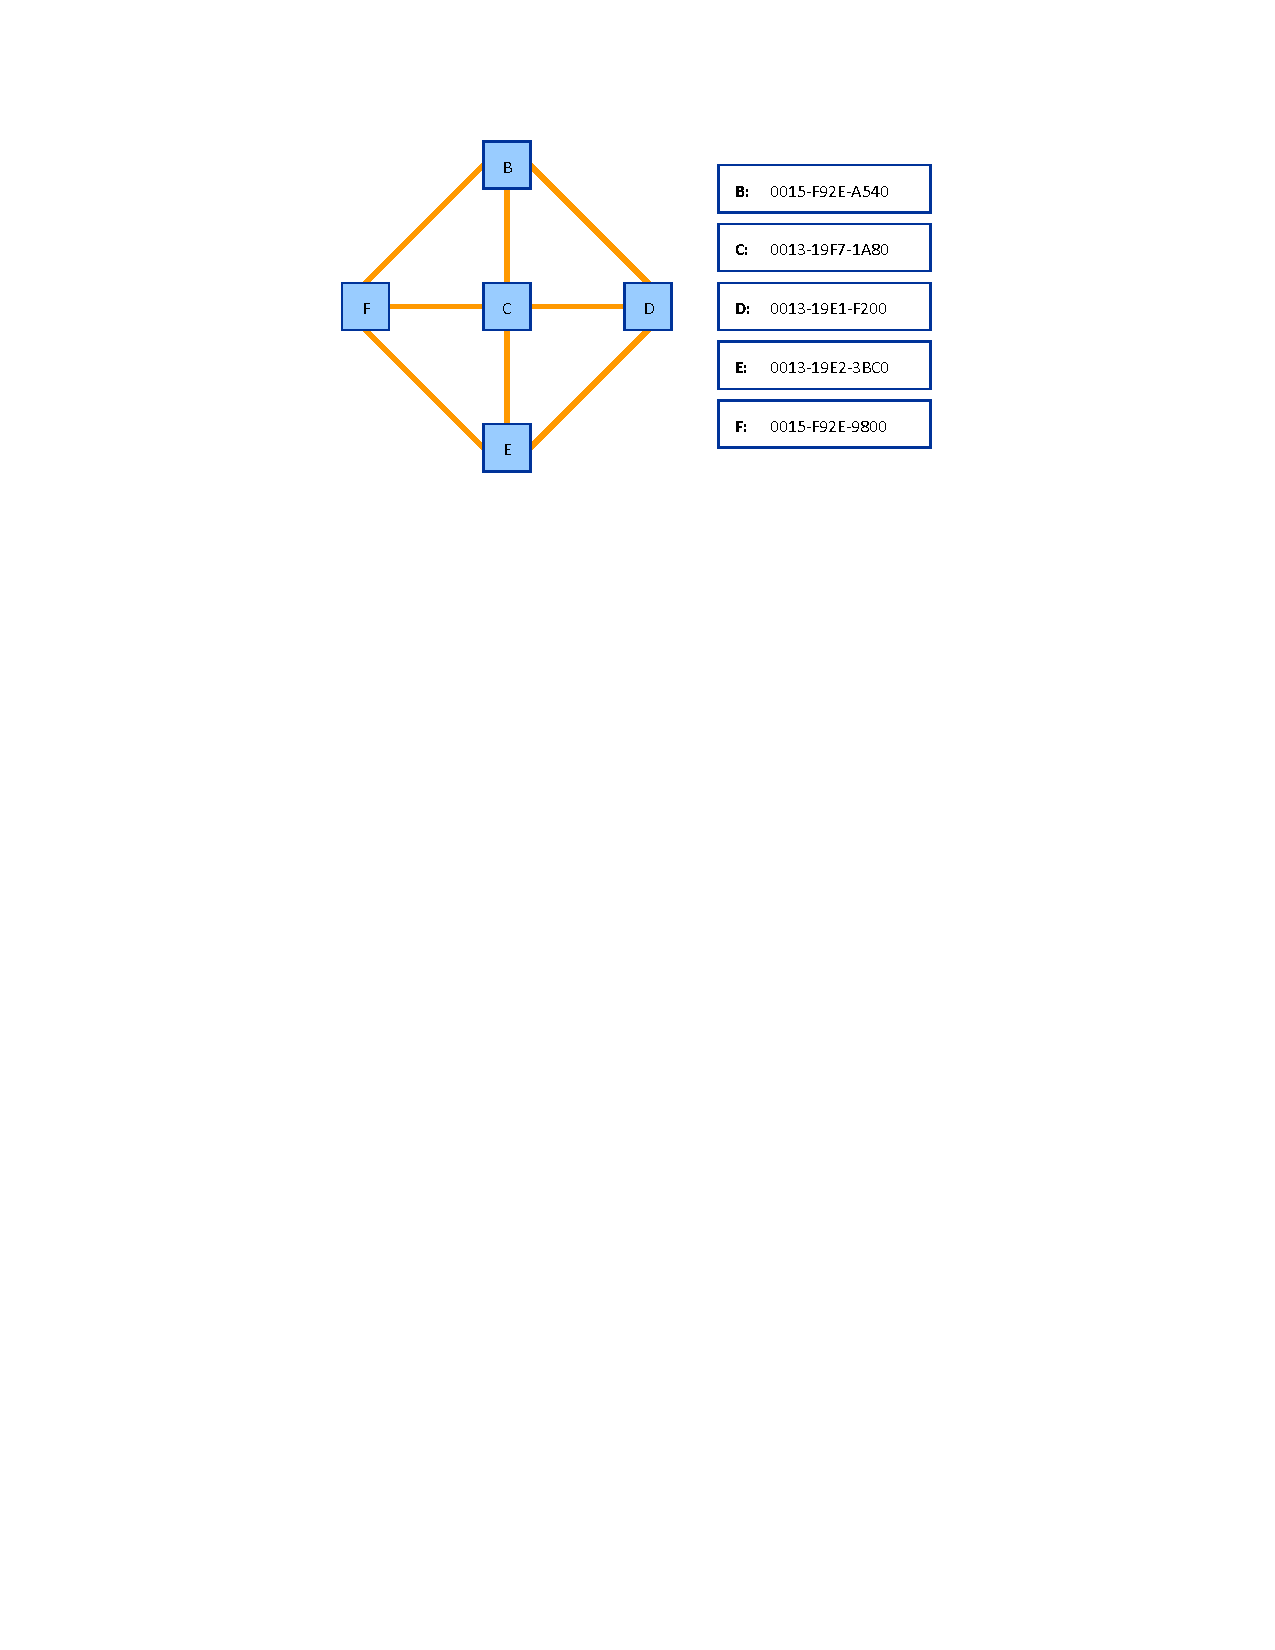
\includegraphics[width=0.9\linewidth]{Figures/StpTopology.pdf}
\else
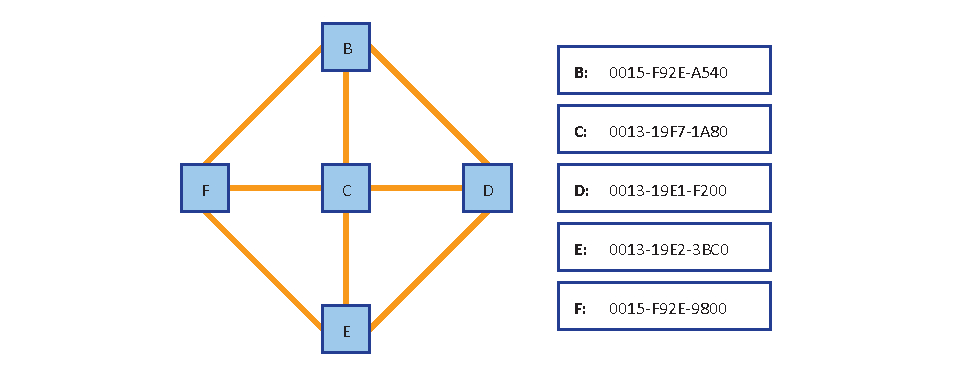
\includegraphics[width=0.9\linewidth]{Figures/StpTopology.eps}
\fi
\caption{The network topology used for the STP practical exercise.}
\label{fig:StpTopology}
\end{figure}

\begin{center}
\sffamily\small
\begin{tabular}{>{\columncolor{tablegray}}p{15cm}}

\multicolumn{1}{>{\columncolor{tableorange}}l}{Questions and Tasks}\\
Find the \texttt{\color{blue}BridgeId} of each switch.\\
\hline
Compute which is the spanning tree and draw it.\\
\hline
Which is the root switch?\\
\hline
Which is the role of each port?\\
\hline
Which are the activated ports?\\
\hline
\end{tabular}
\end{center}

Fill in the table \ref{tab:Stp}.


\begin{table}
\sffamily\small
\centering
\begin{tabular}{>{\columncolor{tablegray}}ccccc}
\multicolumn{1}{>{\columncolor{tableorange}}c}{Switch ID} & \multicolumn{1}{>{\columncolor{tableheader}}c}{MAC} & \multicolumn{1}{>{\columncolor{tableheader}}c}{Port} & \multicolumn{1}{>{\columncolor{tableheader}}c}{Role} &
\multicolumn{1}{>{\columncolor{tableheader}}c}{State} \\
Switch B & 00:15:F9:2E:A5:40 & & & \\
\hline
Switch C & 00:13:19:F7:1A:80 & & & \\
\hline
Switch D & 00:13:19:E1:F2:00 & & & \\
\hline
Switch E & 00:13:19:E2:3B:C0 & & & \\
\hline
Switch F & 00:15:F9:2E:98:00 & & & \\
\hline
\end{tabular}
\caption{The spanning tree.}
\label{tab:Stp}
\end{table}

\section{Practical Verification}

Now you will verify that the STP constructed by the switches is in fact the one you computed in the previous section. Use the VLAN 1 to connect to the five switches (B, C, D, E, F). It is recommended to open five simultaneous Telnet connections, one for each of the switch.

Each group will work in a different VLAN. The teacher will assign a VLAN to each group. Make sure that your VLAN is included in all the trunk ports. Each group will have a different STP, as the network creates a tree for each VLAN.

In each of the switches, enter the \emph{privileged EXEC} mode and use the command:

\begin{lstlisting}
Switch# show spanning-tree vlan <id>
\end{lstlisting}

Observe all the fields and make sure you understand them.

\begin{center}
\sffamily\small
\begin{tabular}{>{\columncolor{tablegray}}p{15cm}}
\multicolumn{1}{>{\columncolor{tableorange}}l}{Question}\\
What can you see?\\
\hline
Find the BridgeId of each switch. Compute which is the spanning tree and draw it.\\
\hline
Which switch is the root? Which is the role of each port? Which ports are activated?\\
\hline
Fill in the table \ref{tab:Stp} and compare practical results to the theoretical computation.\\
\hline
\end{tabular}
\end{center}



\section{Changing the STP Configuration}

Now that you are familiar with the STP parameters, you will make some changes that will result in the computation of a new tree. In the \emph{global configuration} mode use the command:

\begin{lstlisting}
Switch(config)# spanning-tree vlan <id>
\end{lstlisting}
or, alternatively, you may use:

\begin{lstlisting}
Switch(config)# interface vlan <id>
Switch(config)# spanning-tree
\end{lstlisting}
to see which parameters are susceptible to be configured. Use the question mark \texttt{\color{blue}?} to see all the available parameters and make sure you understand them.

The exercise that we propose is to change the priority of one of the switches different from the root switch. The default behavior is that the switch with the lowest MAC address is selected as a root. The reason is that, in the default configuration, the priority of all the switches is 32768. By changing the priority of one of the switches to a lower value, we can force that that particular switch becomes the root.

Go ahead and change the root switch and observe the new configuration of the tree. Fill in the table \ref{tab:Stp} for this new configuration and draw the new tree.

\section{Link Failure}

This exercise cannot be started until all the groups have finished the previous one. If you reach this exercise before the other groups, move on to the next exercise while you wait for all the groups to be ready for the link failure.

Now we will disconnect one of the links to simulate a link failure. Compute in advance your new spanning tree after the link failure. Ask your teacher which is the cable that will be disconnected.

After the disconnection, check which is the new configuration and compare it with the one that you have predicted. Explain what happened.

\section{BPDUs}

Use the computer connected to the VLAN 1 (the computer used for the administration of the switch) and capture the traffic for several seconds using \emph{Wireshark}. Observed the received STP frames and identify the different fields in the packet. Write them down to include them in your report and find out which is the meaning of the information in each of the fields.

\begin{center}
\sffamily\small
\begin{tabular}{>{\columncolor{tablegray}}p{15cm}}

\multicolumn{1}{>{\columncolor{tableorange}}l}{Question}\\
Why are you receiving these frames at your computer?\\
\hline
\end{tabular}
\end{center}

\chapter{Routing}

\section{Home Preparation}

\begin{center}
\sffamily\small
\begin{tabular}{>{\columncolor{tablegray}}p{15cm}}
\multicolumn{1}{>{\columncolor{tablered}}l}{Important}\\
For this practical exercise, you have to submit a report the answers to the questions below. When submitting the answers to the questions, be brief but precise. If you include screenshots, indicate on the screenshot what is the answer.\\
\hline
\end{tabular}
\end{center}

RIP and OSPF are two of the most widely used routing protocols. Find information about these two protocols and compare them. Describe what is the format of a routing table and explain how each of the protocols work.

Read the following quick guide:

\url{www.jaumebarcelo.info/teaching/lxs/routing/GUIA_RAPIDA_CISCO_2010.pdf}

Then, download the router user manuals:

\url{www.jaumebarcelo.info/teaching/lxs/routing/manuals_routers.rar}

\section{First Session}

\begin{center}
\sffamily\small
\begin{tabular}{>{\columncolor{tablegray}}p{15cm}}
\multicolumn{1}{>{\columncolor{tablered}}l}{Important}\\
Each group must select a computer that has a console serial connection.\\
\hline
Start your computer in Windows.\\
\hline
Before disconnecting the computer from the Internet, download the TFTP server from the web site \url{http://tftpd32.jounin.net/}, and save it on one of the computers that you will use to connect to the router.\\
\hline
\end{tabular}
\end{center}

In this first session each group will work with a router. The goals of this session are:
\begin{itemize}
\item Getting familiar with the configuration method.
\item Configuring the Ethernet interfaces.
\item Observe the RIP protocol in action.
\item Save the configuration in an external TFTP server.
\end{itemize}

\begin{figure}
\centering
\ifpdf
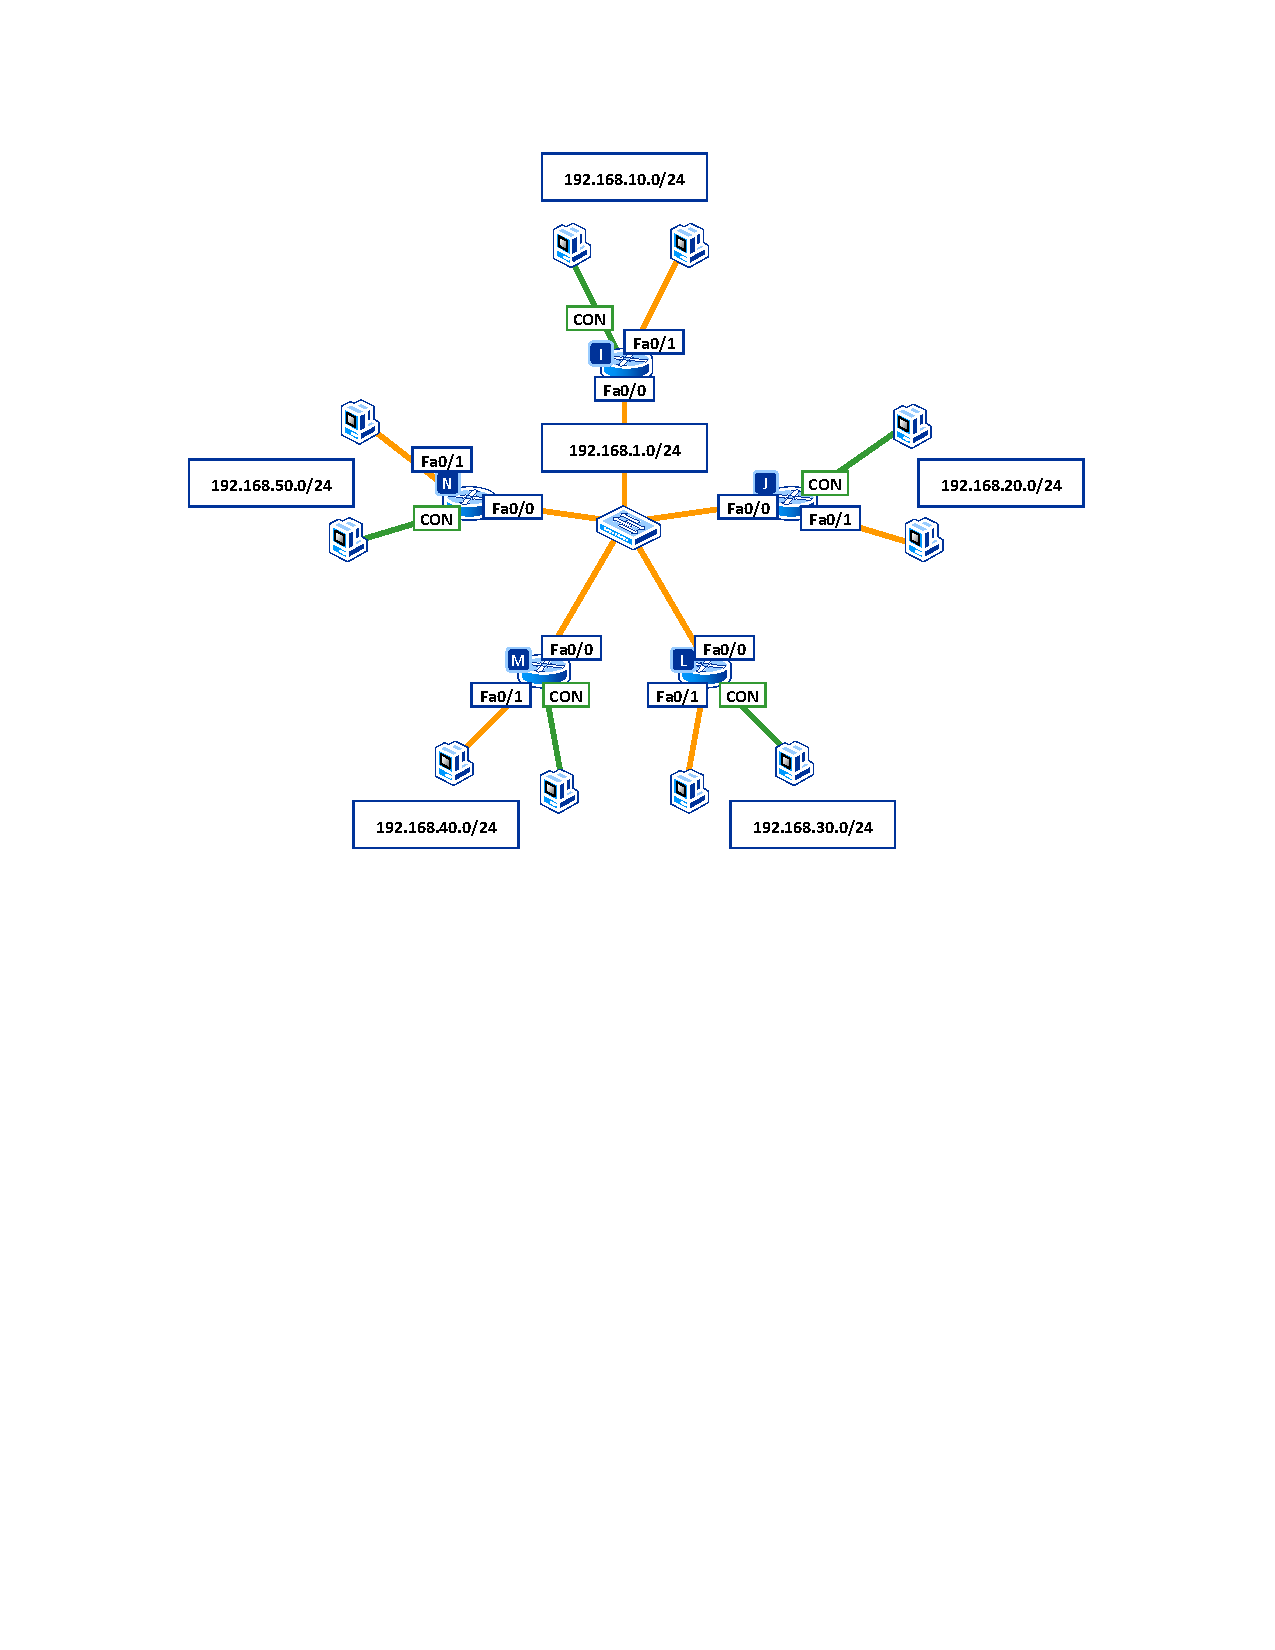
\includegraphics[width=0.9\linewidth]{Figures/RoutingEthernet.pdf}
\else
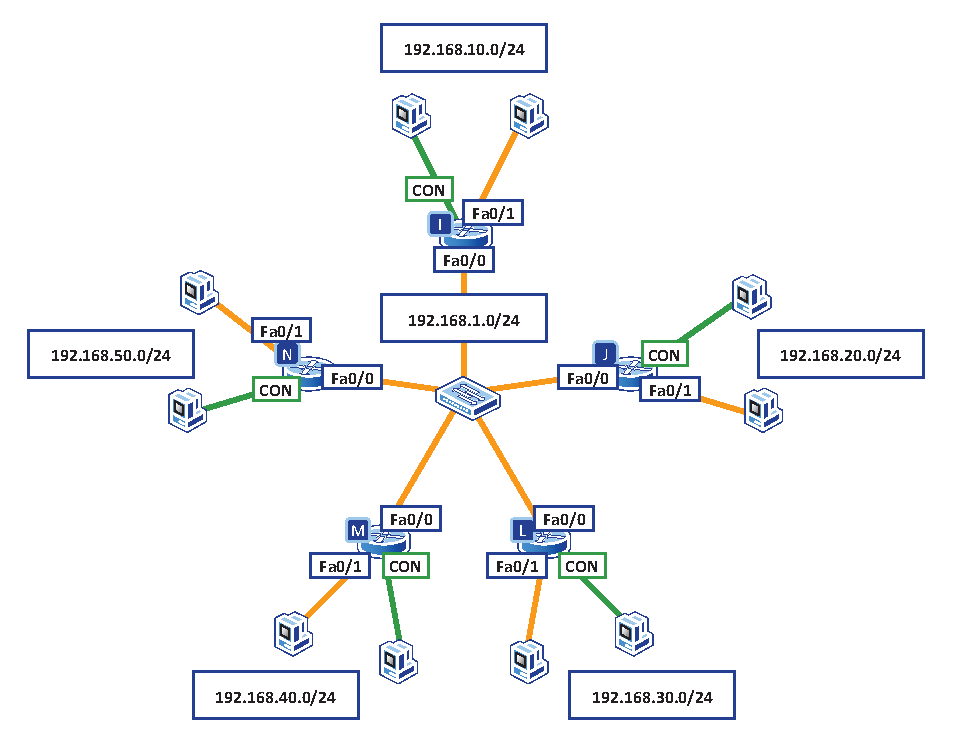
\includegraphics[width=0.9\linewidth]{Figures/RoutingEthernet.eps}
\fi
\caption{The network topology used for the Ethernet routing exercise.}
\label{fig:RoutingEthernet}
\end{figure}

The routers are connected to each other using the Ethernet interfaces and forming the topology from the figure \ref{fig:RoutingEthernet}. Use the console connection to connect to the routers (use \emph{PuTTY} to open a serial connection at 9600 bps). The COM port number (e.g. COM1, COM2, etc.) depends on your computer configuration\footnote{You can see the name of the local serial ports in the \emph{Device Manager} snap-in. To open the snap-in, click on \textsf{Start} \textgreater \textsf{Run...}, type \texttt{devmgmt.msc} and click \textsf{OK}. The serial ports are listed under the \emph{Ports} branch.}. The escape keystroke to exit the \texttt{ping} command in a router is \textsf{Ctrl-Alt-6}.

\subsection{Checking the Router Status}

Use the console to connect to your router and try the following commands. Prepare a summary of what you can see with each command.

\begin{lstlisting}
show history
show protocols
show interfaces
show ip route
\end{lstlisting}

\begin{center}
\sffamily\small
\begin{tabular}{>{\columncolor{tablegray}}p{15cm}}
\multicolumn{1}{>{\columncolor{tableorange}}l}{Questions \textbf{(4 $\times$ 3\,\%)}}\\
For each of the previous commands, what does the output represent?\\
\hline
\end{tabular}
\end{center}

\subsection{Create a Running and Startup Configuration}

Enter the privileged EXEC mode with the command:

\begin{lstlisting}
Router> enable
\end{lstlisting}

and password \texttt{\color{blue}cisco}, and the the global configuration mode

\begin{lstlisting}
Router# configure terminal
\end{lstlisting}

\begin{center}
\sffamily\small
\begin{tabular}{>{\columncolor{tablegray}}p{15cm}}
\multicolumn{1}{>{\columncolor{tableorange}}l}{Tasks \textbf{(4 $\times$ 3\,\%)}}\\
Find and include to your report the commands to:
\begin{itemize}
\item show and change the router name;
\item debugging mode configuration;
\item send pings from the router, and;
\item activate fair queueing on the ethernet interfaces (e.g. FastEthernet0/0).
\end{itemize}\\
\hline
\end{tabular}
\end{center}

Use the following commands to show and save the current configuration to the startup configuration from the privileged mode.

\begin{lstlisting}
Router# show running-config
Router# copy running-config startup-config
\end{lstlisting}

\subsection{IP Addresses Configuration}

Go to your physical router equipment and check which interfaces are visible. Use the following command to see what interfaces are available in the router.

\begin{lstlisting}
Router# show interfaces
\end{lstlisting}

\begin{center}
\sffamily\small
\begin{tabular}{>{\columncolor{tablegray}}p{15cm}}
\multicolumn{1}{>{\columncolor{tableorange}}l}{Tasks \textbf{(5\,\%)}}\\
Include in your report a table with the following information for each interface:
\begin{itemize}
\item the interface name;
\item the interface MTU;
\item the interface bandwidth, and;
\item the encapsulation protocol.
\end{itemize}\\
\hline
\end{tabular}
\end{center}

Enter in the configuration mode of the Ethernet interface with the command:

\begin{lstlisting}
Router(config)# interface <interface name>
\end{lstlisting}

Then, set the IP address to \texttt{192.168.{\color{red}X}0.1}, where \texttt{\color{red}X} is the number of your group. Use a /24 network mask. Use the IP address \texttt{192.168.{\color{red}X}0.2} for the Ethernet interface of your computer.

\begin{center}
\sffamily\small
\begin{tabular}{>{\columncolor{tablegray}}p{15cm}}
\multicolumn{1}{>{\columncolor{tableorange}}l}{Question \textbf{(5\,\%)}}\\
What is the command to configure the IP address on the router interface? Indicate the command mode in which you must execute this command.\\
\hline
\end{tabular}
\end{center}

Use the command:

\begin{lstlisting}
Router# show interfaces
\end{lstlisting}

to verify the IP address assignment, and enable the interface with the command:

\begin{lstlisting}
Router(config-if)# no shutdown
\end{lstlisting}

\begin{center}
\sffamily\small
\begin{tabular}{>{\columncolor{tablegray}}p{15cm}}
\multicolumn{1}{>{\columncolor{tableorange}}l}{Task \textbf{(5\,\%)}}\\
Include in your report the relevant output of at least one command showing that you successfully configured the IP address on the Ethernet interface.\\
\hline
\end{tabular}
\end{center}

Verify the line status and the interface status using the command:

\begin{lstlisting}
Router# show protocols
\end{lstlisting}

Use the commands:

\begin{lstlisting}
Router# show cdp neighbors
\end{lstlisting}

and:

\begin{lstlisting}
Router# show cdp neighbors detail
\end{lstlisting}

to see the neighboring Cisco devices.

\begin{center}
\sffamily\small
\begin{tabular}{>{\columncolor{tablegray}}p{15cm}}
\multicolumn{1}{>{\columncolor{tableorange}}l}{Question and Tasks \textbf{(5\,\%)}}\\
What are the devices displayed by the \texttt{show cdp neighbors} command? Write down the information received from the different interfaces.
\begin{itemize}
\item the neighbor identifier;
\item the IP address, and;
\item the port.
\end{itemize}\\
\hline
\end{tabular}
\end{center}

Use the \texttt{\color{blue}ping} command to test the connectivity to at least one other router in the lab.

\begin{center}
\sffamily\small
\begin{tabular}{>{\columncolor{tablegray}}p{15cm}}
\multicolumn{1}{>{\columncolor{tableorange}}l}{Task \textbf{(5\,\%)}}\\
Include in your report the output of the \texttt{\color{blue}ping} command, indicating the round-trip times.\\
\hline
\end{tabular}
\end{center}

From your computer, use the PuTTY in Telnet mode to connect to your router.

\begin{center}
\sffamily\small
\begin{tabular}{>{\columncolor{tablegray}}p{15cm}}
\multicolumn{1}{>{\columncolor{tableorange}}l}{Questions \textbf{(5 $\times$ 1\,\%)}}\\
Is it possible to remotely configure a router using Telnet?\\
\hline
Is login and password required?\\
\hline
Does a console user notice that there is an ongoing telnet connection?\\
\hline
Use telnet to change a parameter of the router (such as the router name) and verify the changes both using the console and the telnet connection. What happens?\\
\hline
Do any messages appear on the console when changes are done over Telnet? What information is included in these messages?\\
\hline
\end{tabular}
\end{center}

Logout the Telnet session to the Cisco router.

\subsection{IP Routing Configuration}

In this exercise, we shall enable the RIP protocol and check the status of the routing table as well as the RIP transactions of each router.

Check whether IP routing is enabled using the command:

\begin{lstlisting}
Router# show protocols
\end{lstlisting}

\begin{center}
\sffamily\small
\begin{tabular}{>{\columncolor{tablegray}}p{15cm}}
\multicolumn{1}{>{\columncolor{tableorange}}l}{Question \textbf{(5\,\%)}}\\
What is the status of IP routing?\\
\hline
\end{tabular}
\end{center}

Enter the global configuration mode and enter the submenu \texttt{\color{blue}router}.

\begin{center}
\sffamily\small
\begin{tabular}{>{\columncolor{tablegray}}p{15cm}}
\multicolumn{1}{>{\columncolor{tableorange}}l}{Question \textbf{(5\,\%)}}\\
What is the purpose of this submenu?\\
\hline
\end{tabular}
\end{center}

Use the \texttt{\color{blue}?} command to list available routing protocols and write down the results. Enter into the configuration of RIP.

\begin{lstlisting}
Router(config)# router rip
\end{lstlisting}

Use the command:

\begin{lstlisting}
Router(config-router)# network <your network>
\end{lstlisting}

to associate your network to the RIP routing process. Assume that we are working with \emph{C} class IP addresses. Therefore, the last byte of the network address must be 0. Verify that the RIP protocol is now enabled and that your network has been recognized by the router using the command:

\begin{lstlisting}
Router# show ip protocol
\end{lstlisting}

\begin{center}
\sffamily\small
\begin{tabular}{>{\columncolor{tablegray}}p{15cm}}
\multicolumn{1}{>{\columncolor{tableorange}}l}{Task \textbf{(5\,\%)}}\\
Include in your report the output of the previous command showing that the RIP protocol has been enabled.\\
\hline
\end{tabular}
\end{center}

Observe the relevant parameters and answer the following questions:

\begin{center}
\sffamily\small
\begin{tabular}{>{\columncolor{tablegray}}p{15cm}}
\multicolumn{1}{>{\columncolor{tableorange}}l}{Questions \textbf{(3 $\times$ 2\,\%)}}\\
What timers do you identify for the RIP protocol?\\
\hline
What are their values?\\
\hline
What happens if we change the values?\\
\hline
\end{tabular}
\end{center}

Verify the status of the routing table with the command:

\begin{lstlisting}
Router# show ip route
\end{lstlisting}

\begin{center}
\sffamily\small
\begin{tabular}{>{\columncolor{tablegray}}p{15cm}}
\multicolumn{1}{>{\columncolor{tableorange}}l}{Task and Questions \textbf{(3 $\times$ 2\,\%)}}\\
Include in your report the routing table of your router, after the RIP protocol has been enabled on at least one other router in the lab.\\
\hline
What is the meaning of each of the fields in the table?\\
\hline
How do you identify the networks advertised using the RIP protocol?\\
\hline
\end{tabular}
\end{center}

\begin{center}
\sffamily\small
\begin{tabular}{>{\columncolor{tablegray}}p{15cm}}
\multicolumn{1}{>{\columncolor{tablered}}l}{Important}\\
For this assignment you must work together with another group. If there is no other group ready, skip this exercise and come back to it when another group reaches this point.\\
\hline
\end{tabular}
\end{center}

Add a static route to the other group's network. Use the following command from the configuration mode.

\begin{lstlisting}
Router(config)# ip route
\end{lstlisting}

\begin{center}
\sffamily\small
\begin{tabular}{>{\columncolor{tablegray}}p{15cm}}
\multicolumn{1}{>{\columncolor{tableorange}}l}{Task \textbf{(5\,\%)}}\\
Include in your report the command you used to setup a static route.\\
\hline
\end{tabular}
\end{center}

Use the \texttt{\color{blue}traceroute} command from your computer, choosing as destination the computer of another group.

\begin{center}
\sffamily\small
\begin{tabular}{>{\columncolor{tablegray}}p{15cm}}
\multicolumn{1}{>{\columncolor{tableorange}}l}{Question \textbf{(5\,\%)}}\\
Include the output of the traceroute command, indicating the network interfaces traversed by the traceroute ICMP or UDP packet?\\
\hline
\end{tabular}
\end{center}

Use the command:

\begin{lstlisting}
Router# debug ip rip
\end{lstlisting}

to show the RIP messages that are sent and received by the router.

\begin{center}
\sffamily\small
\begin{tabular}{>{\columncolor{tablegray}}p{15cm}}
\multicolumn{1}{>{\columncolor{tableorange}}l}{Questions \textbf{(2 $\times$ 2\,\%)}}\\
What are the source and destination of these packets?\\
\hline
What information do we obtain?\\
\hline
\end{tabular}
\end{center}

\subsection{Saving the Router Configuration in a TFTP Server}

A convenient way to store a router's configuration is using TFTP. We need to install the TFTP server in a computer with connectivity (layer 3 connectivity) to the router. Install the server and configure in which folder you want to save the router's configuration.

In the router, execute the command:

\begin{lstlisting}
Router# copy running-config tftp
\end{lstlisting}

and follow the instructions to enter the TFT server address (this is one of your computers) and the filename that you want to use. In the computer, open the configuration file using a text editor.

\begin{center}
\sffamily\small
\begin{tabular}{>{\columncolor{tablegray}}p{15cm}}
\multicolumn{1}{>{\columncolor{tableorange}}l}{Question \textbf{(5\,\%)}}\\
What is the format of the configuration file saved on your computer? How is the content of this file compared to the configuration file viewed in the router console?\\
\hline
\end{tabular}
\end{center}

To copy the configuration in the TFTP server to the router, there are two different options. Use either the command:

\begin{lstlisting}
Router# copy tftp running-config
\end{lstlisting}

on the server or simply copy and paste on the configuration terminal.

\section{Router Interconnection}

\begin{figure}
\centering
\ifpdf
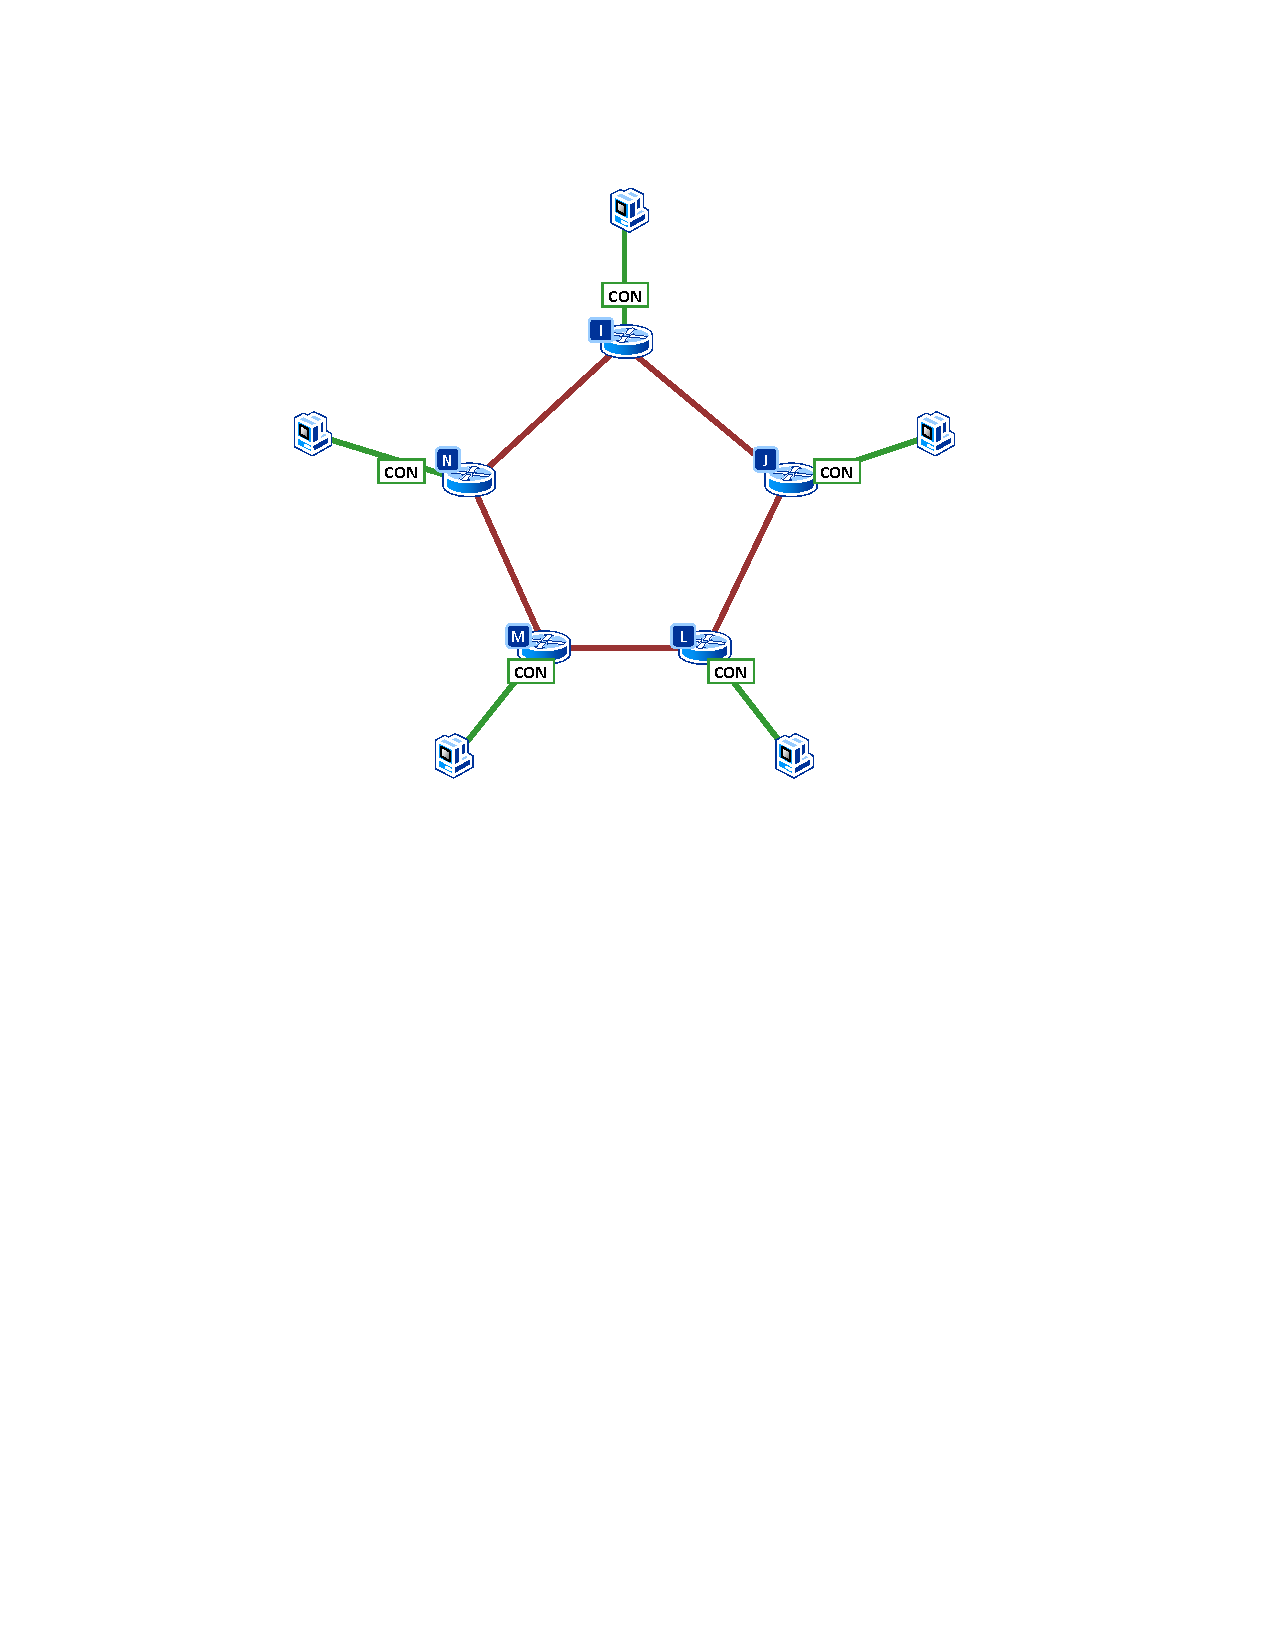
\includegraphics[width=0.9\linewidth]{Figures/RoutingSerial.pdf}
\else
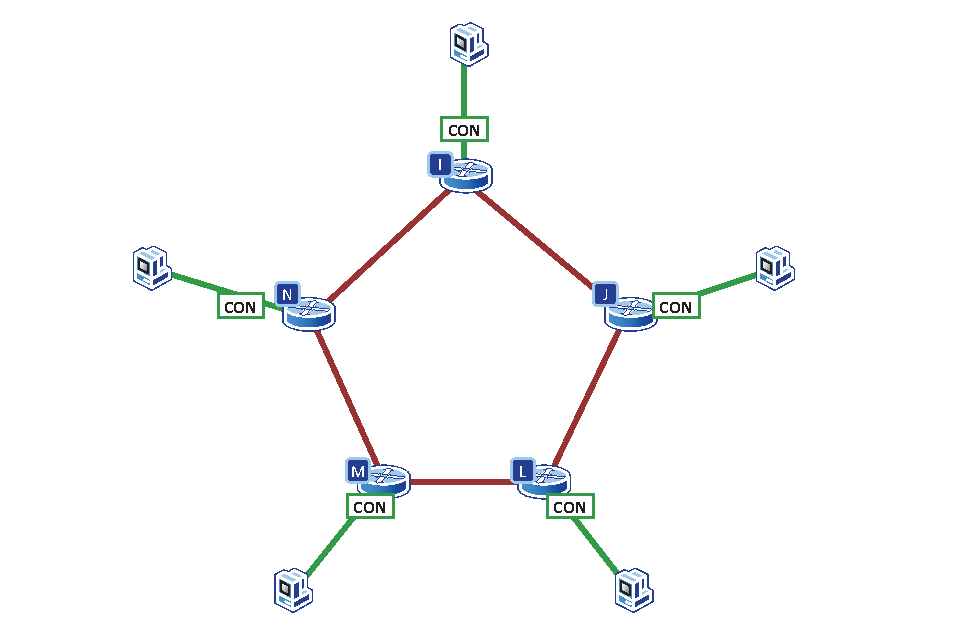
\includegraphics[width=0.9\linewidth]{Figures/RoutingSerial.eps}
\fi
\caption{The network topology used for the WAN routing exercise.}
\label{fig:RoutingSerial}
\end{figure}

In this session, we shall use the WAN (serial) interfaces of the routers. The figure \ref{fig:RoutingSerial} illustrates the topology of the network. In the previous session we used the Ethernet interfaces to connect the routers, and in this session we will use the serial interfaces.

\subsection{Shutdown the Ethernet Interfaces}

{\color{red}\textbf{(10\,\%)}}

Make sure that there is no cable connected to the Ethernet interface, and that there is a cable connecting the serial interfaces. Delete the IP address of the Ethernet interface:

\begin{lstlisting}
Router(config-if)# no ip address
\end{lstlisting}

and administratively shutdown the interface:

\begin{lstlisting}
Router(config-if)# shutdown
\end{lstlisting}

Verify that the changes have been applied using:

\begin{lstlisting}
Router# show running-config
\end{lstlisting}

\subsection{Configuration of the WAN Serial Interface}

{\color{red}\textbf{(50\,\%)}}

From the privileged EXEC mode of your router, enter the global configuration mode. Enter into the configuration of the WAN serial interface and configure the IP.

To choose the IP, use the following algorithm. Assume the your group id is $X$ and your neighbor's group ID is $Y$. If $X<Y$, then your IP is 192.168.XY.1. Otherwise, it is 192.168.YX.2. Use a /30 network mask.

The serial interfaces are interconnected by cables that, in the middle, have male/female connector. The router in the female connector side sets the communication rate. You can find which is the female router issuing the command:

\begin{lstlisting}
Router# show controller
\end{lstlisting}

The DTE interface uses the male connector, and the DCE interface uses the female connector. Alternatively, you may also look at the number on the cable, where 1428 is male and 1429 is female.

Use the command:

\begin{lstlisting}
Router(config-if)# clock rate 128000
\end{lstlisting}

or the closest available rate.

Verify the configuration and use the command:

\begin{lstlisting}
Router(config-if)# no shutdown
\end{lstlisting}

on both connected routers to enable the communication. Then use the command:

\begin{lstlisting}
Router# show protocols
\end{lstlisting}

to verify the state of the line.

Now we will gather information about neighboring devices using the command:

\begin{lstlisting}
Router# show cdp neighbors
\end{lstlisting}

or

\begin{lstlisting}
Router# show cdp neighbors detail
\end{lstlisting}

and we will elaborate a table indicating, for each neighbor, the following information:

\begin{itemize}
\item the neighbor identifier;
\item the neighbor IP address, and;
\item the port.
\end{itemize}

Make sure that routing is enabled using the following commands:

\begin{lstlisting}
Router(config)# ip routing
Router(config)# router rip
Router(config-router)# network 192.168.XX.0
\end{lstlisting}

and look at the routing tables using the command

\begin{lstlisting}
Router# show ip route
\end{lstlisting}

Compare the routing tables to the ones obtained in the previous session and highlight the differences. Use the \texttt{\color{blue}ping} to the other devices in the network.

\begin{center}
\sffamily\small
\begin{tabular}{>{\columncolor{tablegray}}p{15cm}}
\multicolumn{1}{>{\columncolor{tableorange}}l}{Question}\\
Which ones are reachable?\\
\hline
Which ones are not?\\
\hline
Why?\\
\hline
Are there differences in the round-trip-time compared to the measures taken in the previous session?\\
\hline
Why?\\
\hline
\end{tabular}
\end{center}

\subsection{Network Topology}

{\color{red}\textbf{(40\,\%)}}

Prepare a sketch of the network topology that we have used in this session and compare it to the topology of the previous session.

\begin{center}
\sffamily\small
\begin{tabular}{>{\columncolor{tablegray}}p{15cm}}
\multicolumn{1}{>{\columncolor{tableorange}}l}{Question}\\
What are the differences?\\
\hline
What are the advantages?\\
\hline
And disadvantages?\\
\hline
\end{tabular}
\end{center}

\section{Configuration of an L2-L3 Network}

\begin{figure}
\centering
\ifpdf
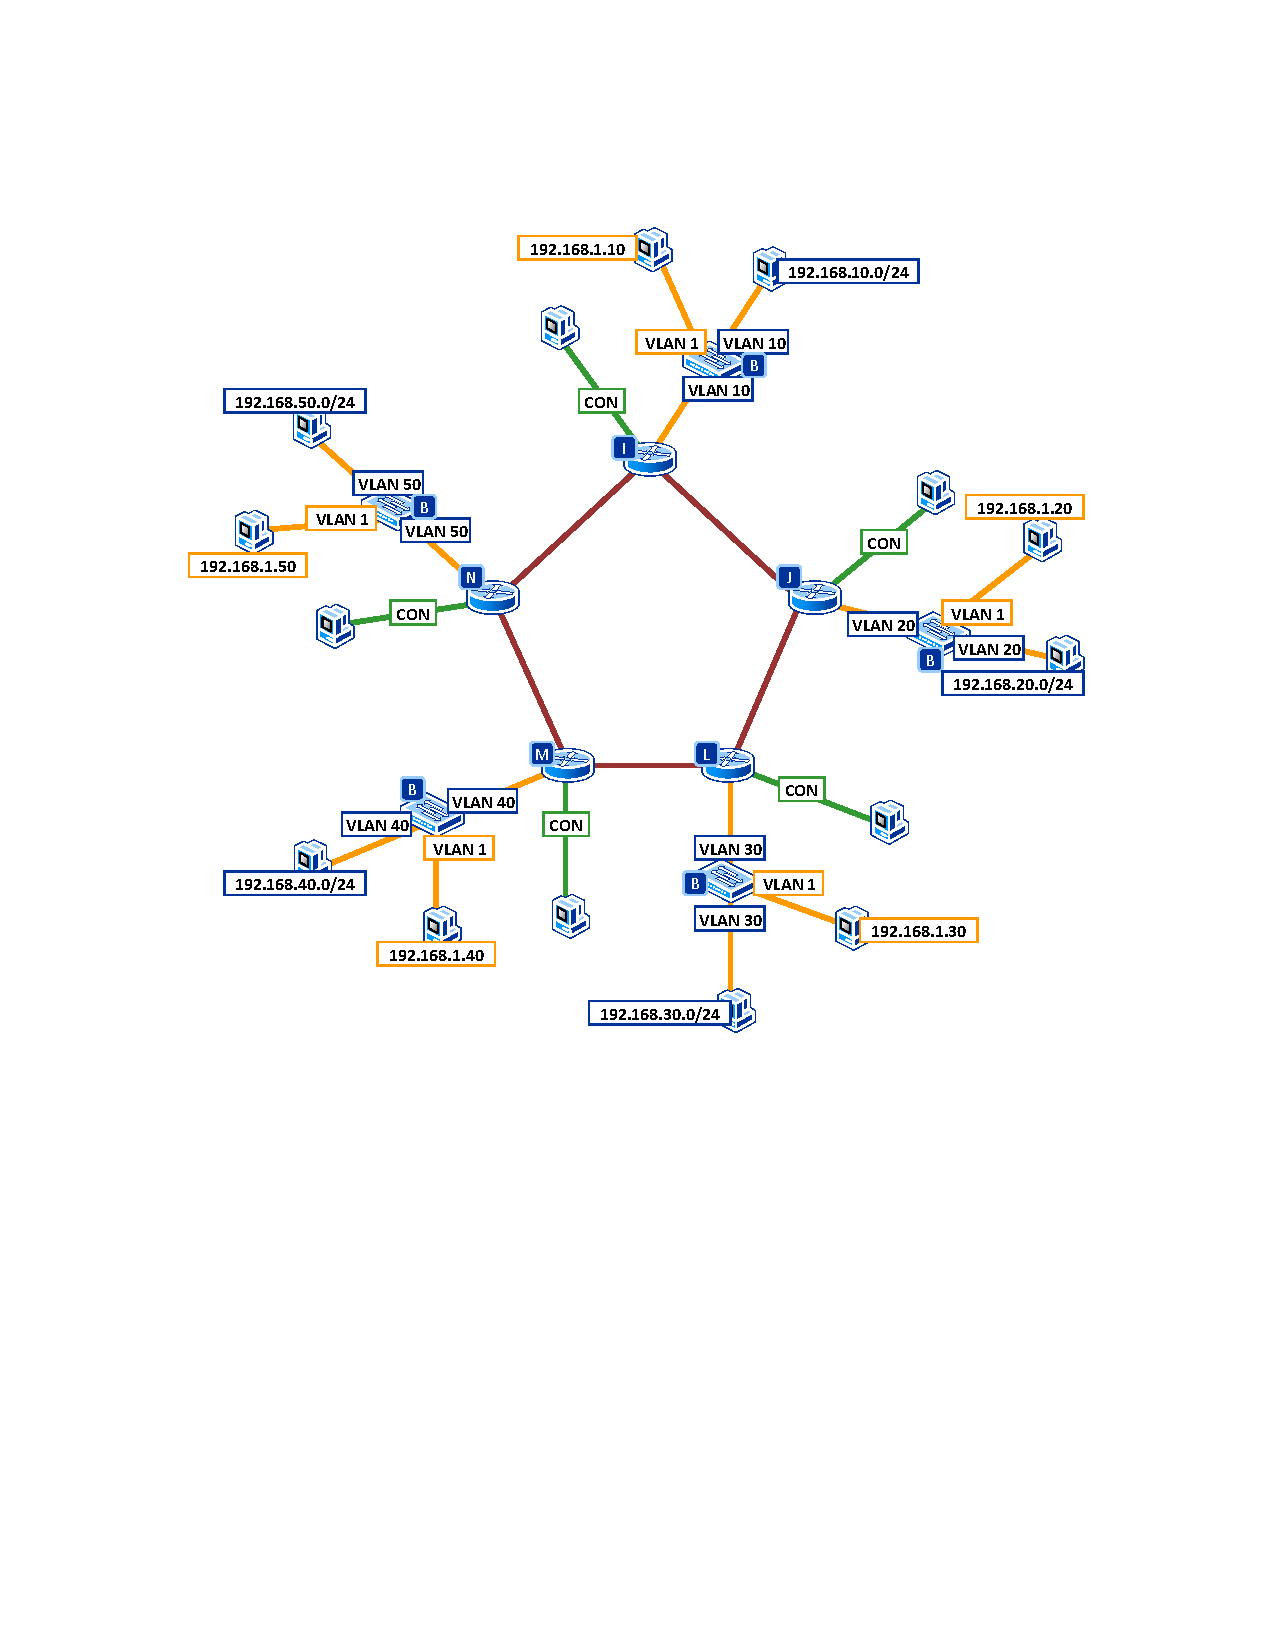
\includegraphics[width=0.9\linewidth]{Figures/RoutingSwitches.pdf}
\else
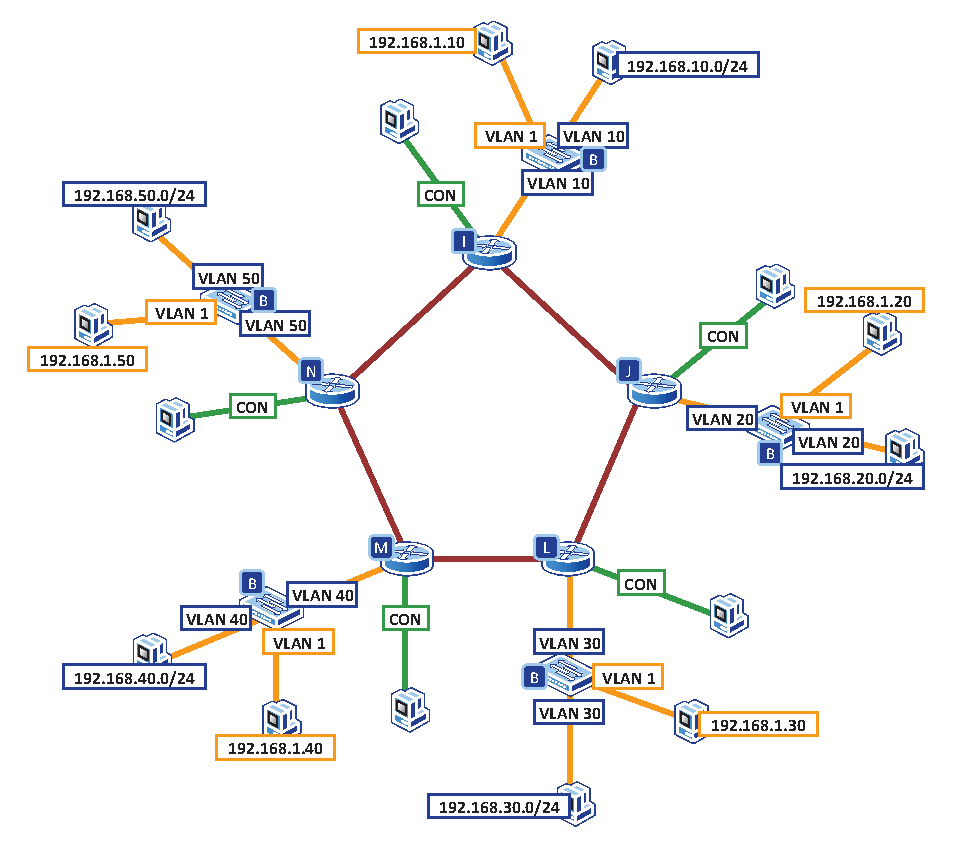
\includegraphics[width=0.9\linewidth]{Figures/RoutingSwitches.eps}
\fi
\caption{The network topology used for the L2-L3 network.}
\label{fig:RoutingSwitches}
\end{figure}

This third session extends the previous one by including switches to the network topology, as shown in the figure~\ref{fig:RoutingSwitches}. The topology consists of a ring of routers connected in a ring using the serial interfaces. Each router is connected using the ethernet interface to a local area network with two or more computers. The devices used in this assignment are:

\begin{itemize}
\item computers;
\item up to six Cisco routers with an ethernet interface and two serial interfaces;
\item up to three Cisco switches, and;
\item direct and cross-over RJ-45 cables.
\end{itemize}

Each group has to configure its router and its VLAN. It is assumed that the previous session has been successfully completed and the connectivity tests were satisfactory.

\subsection{VLAN Configuration}

{\color{red}\textbf{(40\,\%)}}

We connect using Telnet to our switch and enter the privileged EXEC mode. Create a VLAN with a number equal to ten times your group number (e.g. VLAN 20 for group 2). Assign a port connected to the router and one or two other ports connected to computers. Remember to keep the port of the computer you are using for managing the switch in VLAN 1.

Use an IP equal to 192.168.1.XX where XX is the group multiplied by ten for the computer in VLAN 1. Use an IP 192.168.VLAN.YY for the other VLAN. YY is going to be 1 for the router and 2 for the computer. You can use YY equal to 3 if you have another computer.

Test the connectivity between your different computers and with computers of other groups. Write down when a \texttt{\color{blue}ping} command is successful and when it is not successful, and provide an explanation.

\subsection{Configuring the Router LAN Interface}

{\color{red}\textbf{(40\,\%)}}

In the router console enter the privileged EXEC mode and use the command:

\begin{lstlisting}
Router# show interfaces
\end{lstlisting}

to see the interfaces which are available in the router. We enter the global configuration mode and in in the configuration of the LAN (Ethernet) interface. We configure the IP for this interface. Then we enable the interface with the command:

\begin{lstlisting}
Router(config-if)# no shutdown
\end{lstlisting}

and check the link status LED. We can also check the status of the line and the interface using the command:

\begin{lstlisting}
Router# show protocols
\end{lstlisting}

Then we enable the routing. From the global configuration menu we enter the router menu and we use the command:

\begin{lstlisting}
Router(config-router)# network 192.168.VLAN.0
\end{lstlisting}

to associate our network to the routing process. We will assume that we are using class C networks. Then we use the command:

\begin{lstlisting}
Router# show routes
\end{lstlisting}

to see the routing tables.

\subsection{Connectivity Test}

{\color{red}\textbf{(20\,\%)}}

We add our router's IP as as the default gateway for the computers connected to the router. We perform ping tests from the router to the other devices of the network. Finally, we fill in a table with the following information:

\begin{itemize}
\item the destination IP address;
\item the packet loss, and;
\item the average delay.
\end{itemize}

Now we repeat the tests from the computer. If we are on a Linux box, we may also try the \texttt{\color{blue}tracepath} and \texttt{\color{blue}mtr} commands. We will include the configuration of the switch and the router in the lab assignment report.


\chapter{Firewall}

The goals of this assignment include:
\begin{itemize}
\item Familiarizing ourselves with firewalls.
\item Correctly configuring the different options.
\item Configuring a local area network, establishing different security polices using filtering and traffic monitoring.
\item Solve a case study about connecting an SME network to the Internet using a firewall.
\end{itemize}

\section{Home preparation}
Read
\url{www.jaumebarcelo.info/teaching/lxs/ipsec/ASA_Getting_Started.pdf}
and all the assignment, and prepare a solution for the ``case study''.

\section{Configuring the working place}
Each group needs 3 PCs and a Cisco ASA 5505 firewall.

One of the PCs will be connected to the patch panel.
Before disconnecting this PC from the Internet, download an FTP server (e.g. Filezilla)
The other two, are connected to the two internal ports of the firewall.

The firewall and the external PC will be connected to the patch panel and switch B.
The external IP of the firewall will be configured according to the figure (where X is the group number).
Configure the default gateway of the PCs with the corresponding firewall interface (internal for the internal PCs and external for the external PCs).

\begin{figure}
\centering
\ifpdf
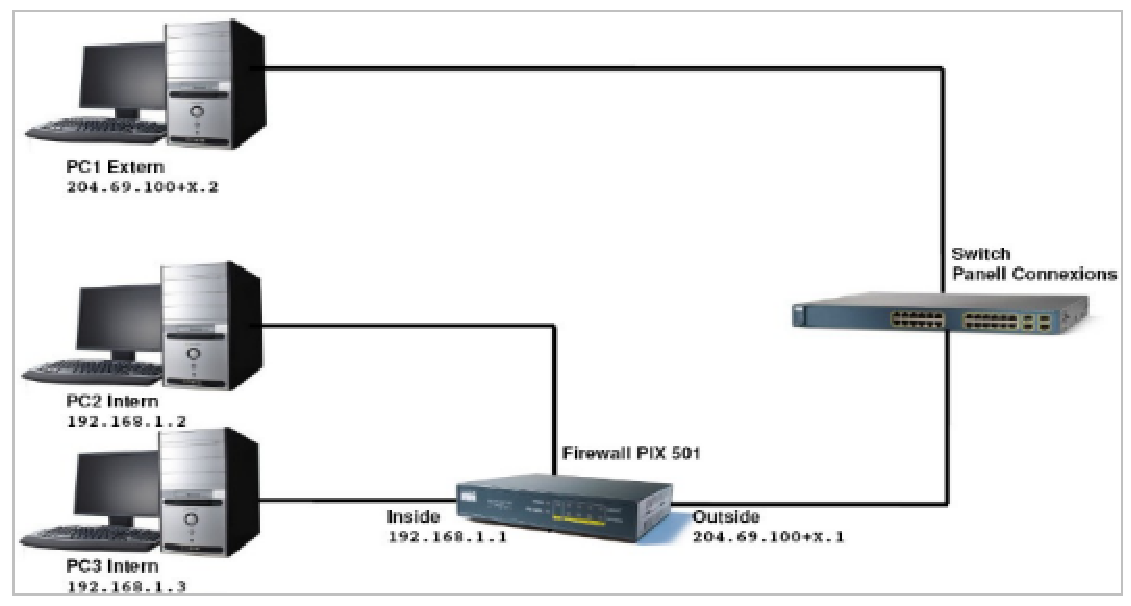
\includegraphics[width=0.9\linewidth]{Figures/firewall_topology.pdf}
\else
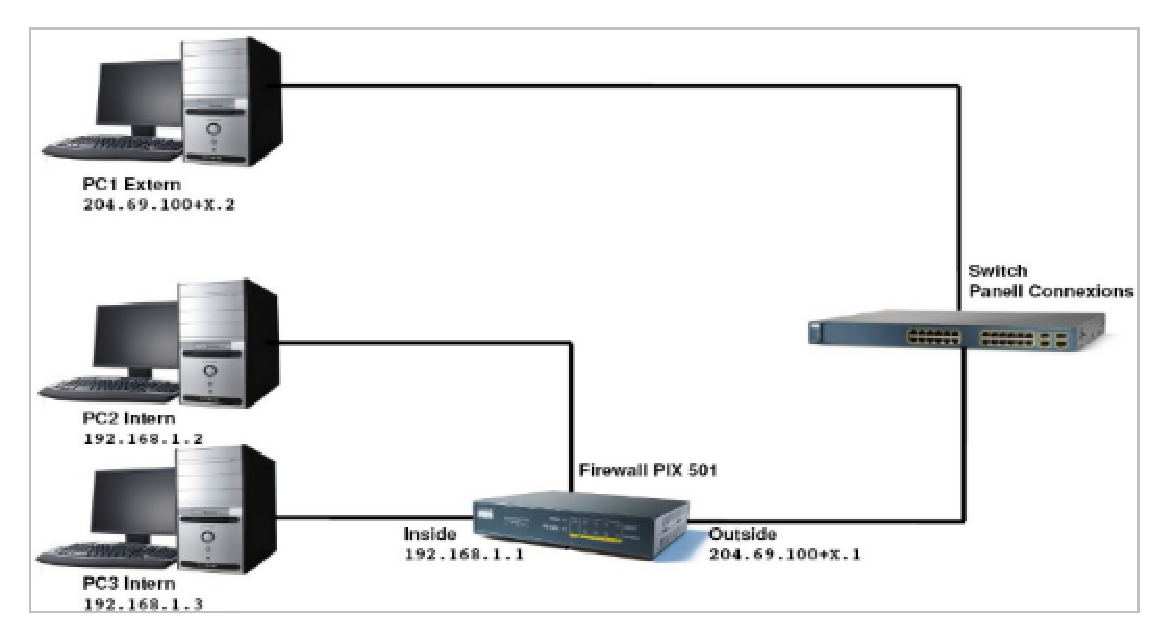
\includegraphics[width=0.9\linewidth]{Figures/firewall_topology.eps}
\fi
\caption{Network topology of the firewalls lab assignment}
\label{fig:firewall_topology}
\end{figure}

We will use FTP to verify that configuration works.
Identify the layer-4 protocol and the port number of FTP.

\section{Adaptive Security Device Manager (ASDM)}

The firewall can be configured using a Java tool which is called Adaptive Security Device Manager (ASDM).
This tool makes it possible to interact with the firewall using a web interface.
Use a windows box to run ASMD.

We will find the ``ASMD launcher'' on the desktop.
The default username and password is blank/blank.
The default IP address is 192.168.1.1 .

The CISCO ASA firewalls assign a ``security level'' to the interfaces.
A security level of 100 means the interface is 100\% trusted.
A security level of 0 means that the interface is not trusted at all.
We will check the interfaces available and their security level.
Discuss the appropriateness of this configuration.

We try to ping between the two PCs connected to the internal interfaces.

\begin{center}
\sffamily\small
\begin{tabular}{>{\columncolor{tablegray}}p{15cm}}
\rowcolor{tableheader}
\multicolumn{1}{>{\columncolor{tableorange}}l}{Question}\\
Does it work? Why?\\
\hline
\end{tabular}
\end{center}

\section{Default configuration of the ASA 5505}
The Cisco ASA use the same OS that the other devices used in the previous assignments, the Cisco IOS.
We will click on options$\rightarrow$preferences and activate ``preview commands before sending them to the device''.
This will show us the equivalent commands that would be used on the console to change the configuration.

Explain which is the default configuration of the firewall.
Observe and explain the different aspects that can be configured using the icons on the left hand side of the screen.

\begin{center}
\sffamily\small
\begin{tabular}{>{\columncolor{tablegray}}p{15cm}}
\rowcolor{tableheader}
\multicolumn{1}{>{\columncolor{tableorange}}l}{Question}\\
What is the default configuration of Ethernet 0/0 (outside)?\\
\hline
Why do you thing that the router ships with this configuration?\\
\hline
\end{tabular}
\end{center}

We will change the address of the Ethernet 0/0 (outside) interface to 204.69.100+X.1. 
Remember that the X is the group number.
We will use a /24 network mask.
Now we connect the outside PC (via switch B) to the outside interface.
We configure the IP of the outside PC to an address of the outside rang and we set the firewall's outside address as the PC's default gateway.

\begin{center}
\sffamily\small
\begin{tabular}{>{\columncolor{tablegray}}p{15cm}}
\rowcolor{tableheader}
\multicolumn{1}{>{\columncolor{tableorange}}l}{Question}\\
Can you ping from the outside PC to an inside PC? Why?\\
\hline
Whats the difference compared to the previous case?\\
\hline
\end{tabular}
\end{center}
Look at the syslog (home screen) to answer this questions.

\section{Firewall}
An alternative configuration option is telnet.
Enable the telnet option 


\backmatter
\bibliographystyle{plain}
\bibliography{Lab,Rfc}
\end{document}
